\documentclass[]{article}
\usepackage{graphicx}
\usepackage{subcaption}
\usepackage[table]{xcolor}


%opening
\title{Multi-Phase Steel Micro-structure Segmentation using UNet: Generalization and Magnification Independence Analysis}
\author{[Early Draft]}

\begin{document}

\maketitle

\begin{abstract}
	
Segmentation of metallographic images plays a critical role in manufacturing processes and quality assessment. This task presents a significant challenge due to the intricate nature of microstructures and the subtle differences among different phases found in Scanning Electron Microscope (SEM) images. Often, these images are processed using off-the-shelf segmentation models without sufficient adaptation to the specific problem requirements. In this paper, we propose an approach that adapts any model architecture, especially UNet,  to meet the unique challenges of steel image segmentation. We demonstrate that the model's performance can be significantly enhanced by carefully selecting and tuning the parameters, rather than relying on pre-configurations. We also highlight the importance of data augmentation and precise labeling in segmentation tasks. For the first time, we propose the use of Electron Backscatter Diffraction (EBSD) images for multi-phase segmentation and introduce a new loss function, SteelSegLoss, which effectively addresses the issues of capturing complex microstructures in images. Finally, we are the first to conduct a scalability experiment, testing our model on different magnification and steel type images, thereby demonstrating its robustness and potential for practical application. Our findings offer valuable insights and practical solutions that can bolster industrial applications and contribute to the ongoing development of AI-driven solutions in the manufacturing industry.

\end{abstract}

\section{Introduction}

The advent of Artificial Intelligence (AI) has brought about transformative changes across various sectors, including manufacturing processes \cite{russel2010}. AI systems, by encapsulating significant knowledge into models, have become an indispensable component of the Industry 4.0 revolution \cite{lasi2014industry}. In this scenario, the segmentation of metallographic images is pivotal for understanding material characteristics and refining manufacturing procedures, thereby enhancing product quality assessment and fostering the creation of new products \cite{gonzalez2008digital, cv_algandapp}.

Among the various applications in industrial manufacturing, our focus is on the segmentation of metallographic images. Image segmentation, a fundamental problem in computer vision, involves dividing an image into distinct regions based on specific criteria \cite{HARALICK1985100}. This problem has been extensively studied and finds applications in numerous domains, including medical image analysis \cite{Litjens_2017, shen2017}, autonomous driving \cite{chen2017deeplab}, and robotics \cite{garciagarcia2017review}.

Initial approaches included patch classification and Class Activation Mapping (CAM). However, these methods are time-consuming and yield rough results. Previously, Optical Microscopy (OM) images were used for analysis, and simple image processing could enable automatic segmentation. However, as we are now entering the stage of developing Mega- and Giga- steels, the analysis targets Scanning Electron Microscope (SEM) images. This makes the given image segmentation problem very challenging due to the intricate nature of steel microstructures and the similarity in appearance among different components when observed under varying magnifications.

Transformation-induced-plasticity (TRIP) effect, is a material phenomenon that occurs in multi-phase microstructures of steel plates. The TRIP effect involves the transformation of retained austenite to martensite during plastic deformation, leading to a significant increase in the work-hardening rate \cite{tripSteels}. This transformation strengthens the neck region, delaying further deformation and enhancing the strength-ductility balance \cite{ALLAIN2004158}. Harnessing the TRIP effect in advanced high-strength steels (AHSS) has emerged as a significant strategy for the steel and automotive industries to maintain high strength and safety properties, while also addressing critical environmental concerns such as fuel consumption and air pollution \cite{BOUAZIZ2011141}. So it becomes essential to find the proper structures of the parts that underwent TRIP effect to access the quality of the produced AHSS. 
One of the ways to finding the structures in the steel to use obtain images using a Scanning Electron Microscope (SEM) and then generate corresponding labels using methods like Electron Backscatter Diffraction (EBSD). Despite its effectiveness, relying solely on EBSD for routine quality assessment presents several challenges. First, EBSD is not only time-consuming and labor-intensive, but it is also cost-prohibitive for large-scale or frequent analysis. Moreover, while EBSD provides detailed crystallographic information, its resolution is often lower compared to SEM, thus limiting its utility for fine-detail microstructural analysis. Moreover previously EBSD maps were only used in dual phase steel image segmentation\cite{ebsd1, ebsd2} and not in multiphase steel structures. Given these challenges, there is a compelling need for alternative, more efficient methods for microstructure characterization. We look towards medical image segmentation for motivation as it also deals with complex and intricate structures that require high precision and accuracy in segmentation. In the medical field, various segmentation models are being applied, most of which are based on UNet due to its ability to perform high-resolution, high-precision image segmentation. However, off-the-shelf UNet models are susceptible to overfitting, necessitating measures to mitigate this issue.

The learning process requires precise labeling for segmentation and it difficult to train the model just on EBSD output results. Often times than not manual supervision is required for consistent images which is time consuming and exhaustive. Furthermore, during manual supervision, interpretations of phases can vary among experts, as these are influenced by individual perspectives and levels of experience. This can lead to discrepancies in the labeling process, making it difficult to achieve universally agreed-upon segmented images. Not to say that this process is prone to human error. Despite the expertise of the individuals involved, inconsistencies may arise due to fatigue, oversight, or subjective interpretation of the images. We therefore use our very own developed Superpixel labeling software tool on top of EBSD images to obtain high resolution and consistent label images. 

\begin{figure}[ht]
	\centering
	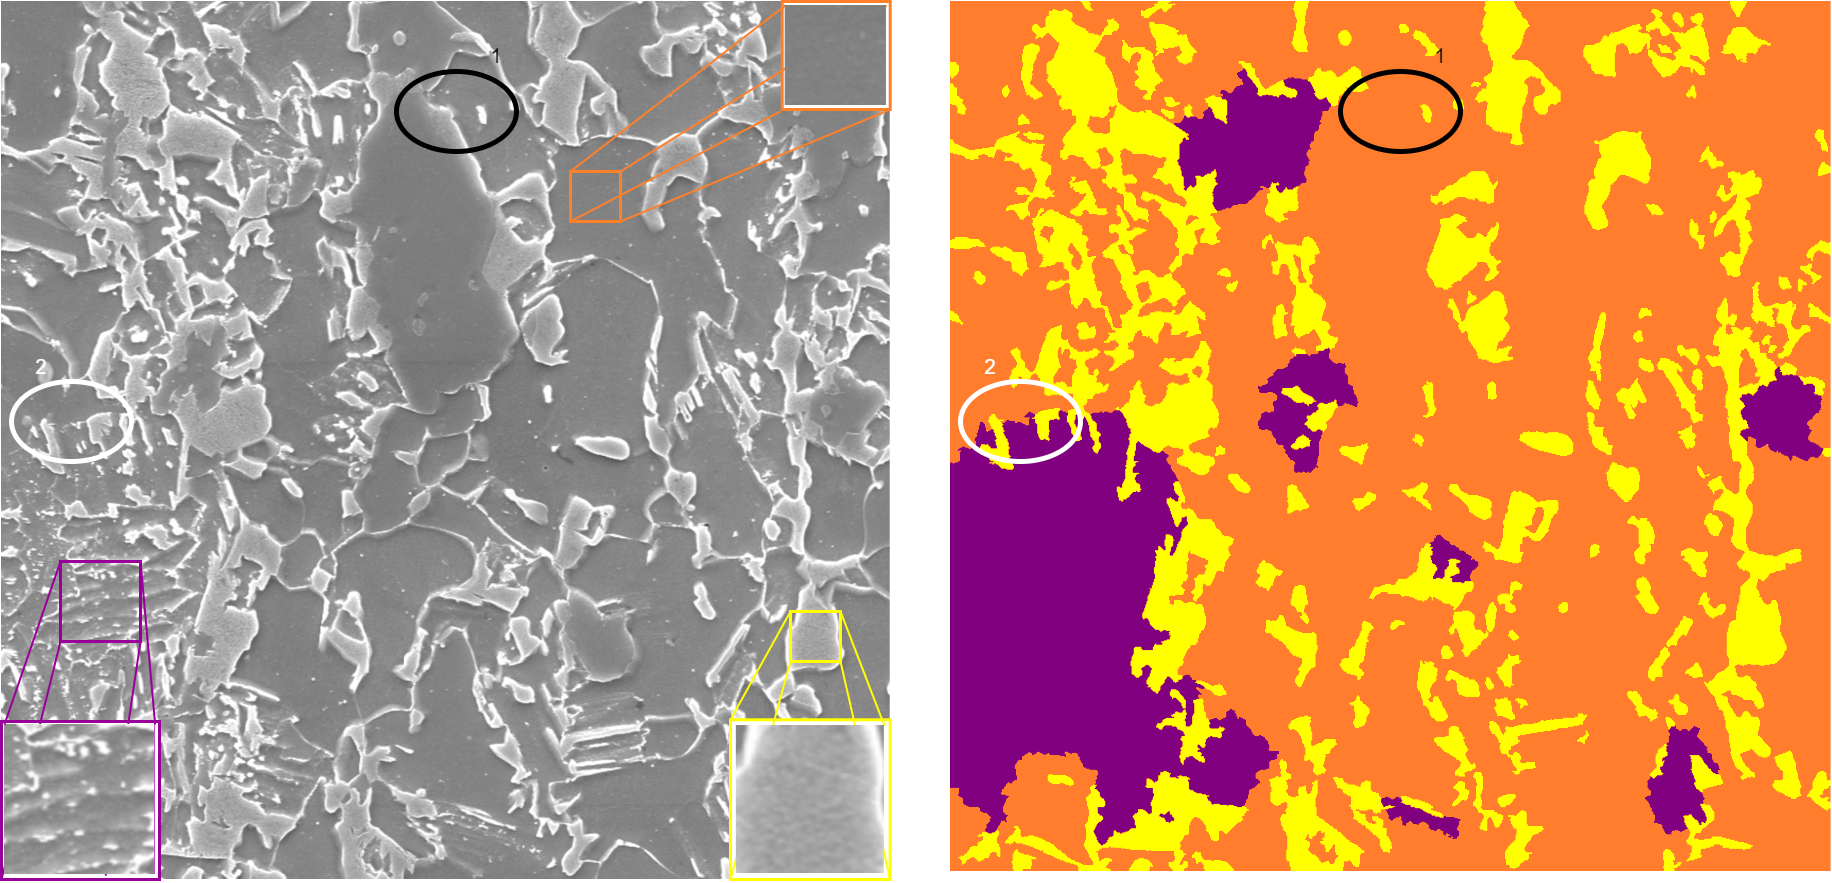
\includegraphics[width=\textwidth]{images/sem-explain2.png}
	\caption{x2700 magnified SEM image of E type steel and corresponding label image made using EBSD and superpixel tool containing 3 phases denoted by three color labels.}
	\label{fig:image-explain}
\end{figure}

The segmentation of microscopic steel images is a challenging task due to the intricate nature of steel microstructures and the similarity in appearance among different components when observed under varying magnifications. Unlike general image segmentation problems where objects have distinct boundaries, the components in steel microstructures often exhibit subtle differences and complex structures that require careful analysis for accurate segmentation \cite{NIPS2012_imagenet} as can be seen in fig \ref{fig:image-explain}. The image contains three different classes, each corresponding to a different phase of the steel microstructure. The labeling colors for each class are as follows:
\begin{itemize}
	\item Orange: Ferrite
	\item Purple: Bainite
	\item Yellow: Martensite
\end{itemize}
 It can be seen that Ferrite (orange) and Martensite (yellow) phases have definitive textures and can be classified into their corresponding labels. However, the Bainite phase (purple) lacks such definitive texture or a clear pattern of occurrence, thereby complicating the segmentation task. Additionally, the black region in the figure underscores the challenge of boundary separation in the SEM image when the label image does not provide clear demarcation. On the other hand, the white region demonstrates a situation where the SEM image does not clearly differentiate class edges, yet the label image shows clear separation. These irregularities in phase boundaries further escalate the complexity of the segmentation task. Since steel microstructures contain critical information about the mechanical properties and quality of the material, it is essential to accurately separate and identify the different components. This level of detail and precision is particularly crucial in applications such as additive manufacturing, quantitative analysis, and quality control.


In this study, we propose the following,
\begin{itemize}
	\item use of EBSD images for multi phase segmentation for the first time.
	\item show various ways in which the UNet models can be configured so as to obtain a superior result instead of using off-the-shelf model.
	\item Propose a new loss function - SteelSegLoss, which addresses the issues of capturing complex microstructures in images. 
	\item Finally we are the first to conduct the scalability experimentation by testing the learned model on different magnification and steel type images unknown to the model to show that it learns the intended microstructures and segments accordingly.
\end{itemize}
 

The subsequent sections of this paper elaborate on our proposed methodology and present experimental results demonstrating its effectiveness in automating microstructure characterization. Section 2 reviews related works in the domain. Section 3 discusses the characteristics and challenges of microstructure segmentation, as well as discusses the image preparation and its properties. Section 4 presents the methodology , including importance of data augmentations and ways in which a UNet model can be modified to suit the problem statement. Section 5 focuses on experimentation, covering evaluation metrics, experimental setup, results on both training and inference images and ablation studies. Section 6 provides a detailed discussion and analysis of the experimental results, addressing challenges and limitations. Finally, section 7 concludes by summarizing the key findings, emphasizing the importance of accurate microstructure segmentation.


\section{Related Works}

Deep learning techniques, particularly convolutional neural networks (CNNs), have shown promising results in various image segmentation tasks. The UNet architecture, a type of CNN, has been widely adopted for medical image segmentation due to its ability to capture both local and global context using a symmetric encoder-decoder structure \cite{cao2021swinunet}.

In the realm of microstructure segmentation, previous studies have explored various methodologies to achieve accurate classification and segmentation results. Velichko et al. proposed a method based on data mining techniques, specifically extracting morphological features and utilizing a feature classification step using Support Vector Machines (SVMs). This approach was applied to cast iron and demonstrated the potential of machine learning in microstructural analysis \cite{sym13071176}. However, this method, while effective for simpler microstructures, may not be as efficient for complex steel microstructures due to their intricate nature and subtle differences among different components.

Similarly, Pauly et al. adopted a similar approach on a contrasted and etched dataset of steel acquired through SEM and LOM imaging \cite{LAI2009665}. However, the results yielded a relatively low accuracy of 48.89% in microstructural classification due to the complex nature of substructures and the lack of discriminative features. This highlights the need for a more robust and efficient method for microstructure segmentation.

Durmaz et al. proposed a multidisciplinary deep learning approach that equally considers specimen preparation and imaging \cite{Durmaz2021}. They trained distinct UNet architectures with 30-50 micrographs of different imaging modalities and electron backscatter diffraction-informed annotations. The study focused on the challenging task of lath-bainite segmentation in complex-phase steel, achieving accuracies of 90% that rival expert segmentations. While this approach has shown promising results, it requires a large number of annotated images for training, which may not always be feasible in practical scenarios.

Recently, \cite{ebsd1, chaurasia23} used UNet for segmenting dual phase steel structures. The papers received good results due to the presence of clear distinction of the classes during classification and segmentation. As the texture of the classes in the images were very different and less ambiguous, it became comparatively easier task to differentiate between the two. The task of multi phase segmentation is comparatively difficult due to ambiguity between the classes. Therefore it is not only important to find texture but also the shape and structure in the microstructures.

Although, \cite{LUENGO2022232} is quite similar to the problem that we are solving, in fact, the paper lays down some concrete foundational research in the domain of steel segmentation. Although they also address the issue of multi phase segmentation, the MetalDAM dataset does not contain EBSD label images, rather label images were produced by using binary mask as pre-annotations before being modified by industry experts. But the labeling process of such intricate details is very subjective and prone to errors. Furthermore, their model does not seem to be scalable. Nevertheless, we drew many inspirations from the paper for our research. We also draw a comparison between the results of MetalDAM and UCHS dataset with our model and proposed augmentations

In contrast to these previous works, our proposed method aims to segment multi phase images that provide a scalable solution when trained only a small number of annotated images using modified available models. We leverage different augmentation strategies to increase the diversity of our training data, thereby enhancing the robustness and generalizability of our model, use a new loss function that has not been used in such task to the best of our knowledge and furthermore, handle image scalability when used on different magnified images and steel types, making it more versatile and applicable to a wider range of scenarios. In summary, while previous studies have made significant contributions to the field of microstructure segmentation, our work aims to address the limitations of these methods by proposing a scalable, efficient, and versatile solution for steel microstructure segmentation.


\section{Background}

\subsection{Motivation and Challenges}
More often than not, people just use off-the-shelf models that are good in segmentation on a given problem without any prior modifications. While convenient, it may not always yield the best results due to the unique characteristics and challenges associated with specific characteristics of the underlying problem statement. In recent times models based on UNet have been the center of attention because of their ability to perform better in segmentation related tasks. The UNet architecture is characterized by its U-shaped design, which consists of a contracting path to capture context and a symmetric expanding path that allows precise localization. This design enables the model to preserve fine-grained details while capturing global context, making it suitable for steel microstructure segmentation. Another key feature of UNet is the incorporation of skip connections, which allow the fusion of features from multiple scales. Each of the UNet models have their own set of unique characteristics and upon modifying certain parameters it can be tuned and adapted to any specific requirement across a wide range of applications, including medical imaging and materials science.

While there are newer variants of UNet that offer improved performance, our objective in this study is not solely to achieve the best possible segmentation results. Instead, we aim to adapt the UNet model specifically for the task of steel image segmentation. We seek to explore and demonstrate how various parameters of the UNet model can be modified to better suit the unique requirements of this task. The modifications we propose and the insights we gain from this process are not limited to the stock UNet model. They can be applied to the newer variants of UNet as well, given that these models are built upon the same foundational principles as the original UNet. By starting with the stock UNet, we provide a baseline that can be easily understood and built upon by researchers and practitioners in the field.

Data augmentation plays a crucial role in improving the performance of deep learning models, particularly in scenarios where the available dataset is limited or imbalanced. By artificially expanding the dataset through various transformations, data augmentation can enhance the model's ability to generalize and reduce overfitting. However, the choice of augmentation techniques should be guided by the problem at hand. In the context of steel image segmentation, the augmentation strategies should be designed to capture the complex textures and structures of different steel phases.

In the specific problem of identifying the different phases, differentiating between the Martensite and Ferrite phases is primarily based on texture, while the identification of the Bainite phase requires capturing shape and patterns, i.e., learning the structure of the underneath microstructures. This dual requirement of learning both texture and structure adds an additional layer of complexity to the segmentation task. As stated before in fig \ref{fig:image-explain}, presence of irregularities when the phases separate is also another issue that needs to be addressed. The absence of landmark information in these images limits the availability of unique characteristics that could aid in capturing the distinct features of microstructures \cite{LUENGO2022232}. Due to the heterogenous material properties in these metallographic images, accurately delineating and classifying different regions becomes difficult. Heterogenous properties also heighten the variations in scale and magnification, leading to changes in the appearance and size of the microstructures.

Class imbalance is another significant challenge in steel image segmentation. When certain classes are underrepresented in the training data, the model may develop a bias towards the majority classes, leading to poor performance on the minority classes. In our case, the presence if Ferrite largely overshadows Bainite in most cases, therefore addressing class imbalance is crucial to ensure that the model accurately segments all classes, regardless of their prevalence in the training data.

Finally, it is essential to test the model on different magnification and types of steel images than the images it was trained on. This step is crucial to evaluate the model's generalizability and its ability to adapt to new, unseen data. By testing the model on a diverse set of images, we can gain a more comprehensive understanding of its performance and identify areas for further improvement.

While manual annotation of metallographic images is a labor-intensive and time-consuming, producing EBSD images is cost-prohibitive and not suitable for more frequent analysis. As a result, there is a scarcity of large, labeled datasets specifically tailored for microstructure segmentation \cite{Roberts2019}. This limitation hinders the application of supervised learning methods, which typically require ample training data to achieve optimal performance.

\subsection{Image Preparation and Properties}
The steel images used in this study is termed 590DP, which signifies a dual-phase steel with a tensile strength of 590MPa. This kind of steel, also known as gigasteel when the tensile strength reaches 1GPa, is classified as ultra-high-strength steel and is commonly used in automotive applications due to its exceptional strength and formability.
The dataset consists of six E-type steel images captured through a Scanning Electron Microscope (SEM). Due to the minuscule size of the phases in this type of steel, using optical microscopy (OM) for image capture is ineffective. Thus, SEM provides the necessary resolution and detail for effective analysis. Corresponding to each SEM image, we generated ground truth labels using Electron Backscatter Diffraction (EBSD), providing precise information about the distinct components and phases present within the steel microstructures.
Labeling of the SEM images was assisted using a superpixel labeling method. Superpixel segmentation groups pixels into larger, coherent superpixels based on similarity in color, texture, and other factors, thus providing a more efficient and accurate labeling process for our dataset. This approach, coupled with the precision of EBSD imaging and the detailed phase information from SEM, ensures the creation of a robust and comprehensive dataset for training and testing our UNet segmentation model.

In the training phase of our study, we utilized five out of the six E-type steel images to augment and train the UNet model. The remaining image served as an initial testing ground to validate the model's learning.

To evaluate the model's performance and its ability to generalize, we extended our testing to include steel images magnified at higher magnifications of 3000x and 5000x. The ability to accurately segment images at these higher magnifications is crucial, as it enables the detailed analysis of complex microstructures that are typically observed at these scales.

Furthermore, to test the model's versatility and its effectiveness across various steel types, our testing dataset was expanded to include images of A-type, H2-type, and D3-type steels. These additional steel types have unique microstructural characteristics that pose different challenges to image segmentation. By testing the model across these diverse types of steel, we aim to validate its robustness and its potential for broad applicability in industrial settings.

\begin{figure}[ht]
	\centering
	\begin{subfigure}[b]{0.2\textwidth}
		\centering
		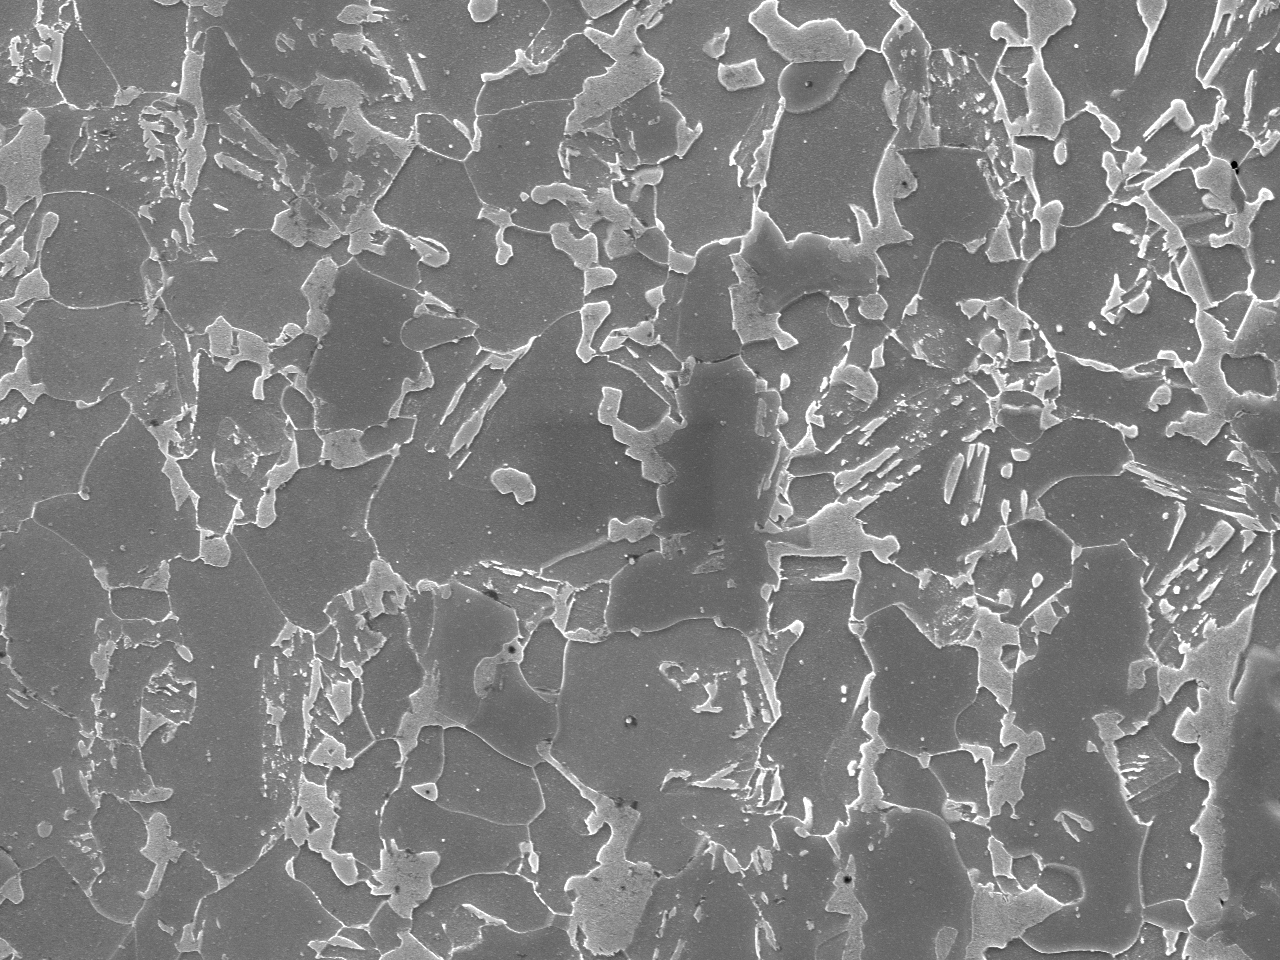
\includegraphics[width=\textwidth]{images/x3000/1.png}
		\caption{x3000 SEM}
		\label{fig:image2.1.1}
	\end{subfigure}
	\begin{subfigure}[b]{0.2\textwidth}
		\centering
		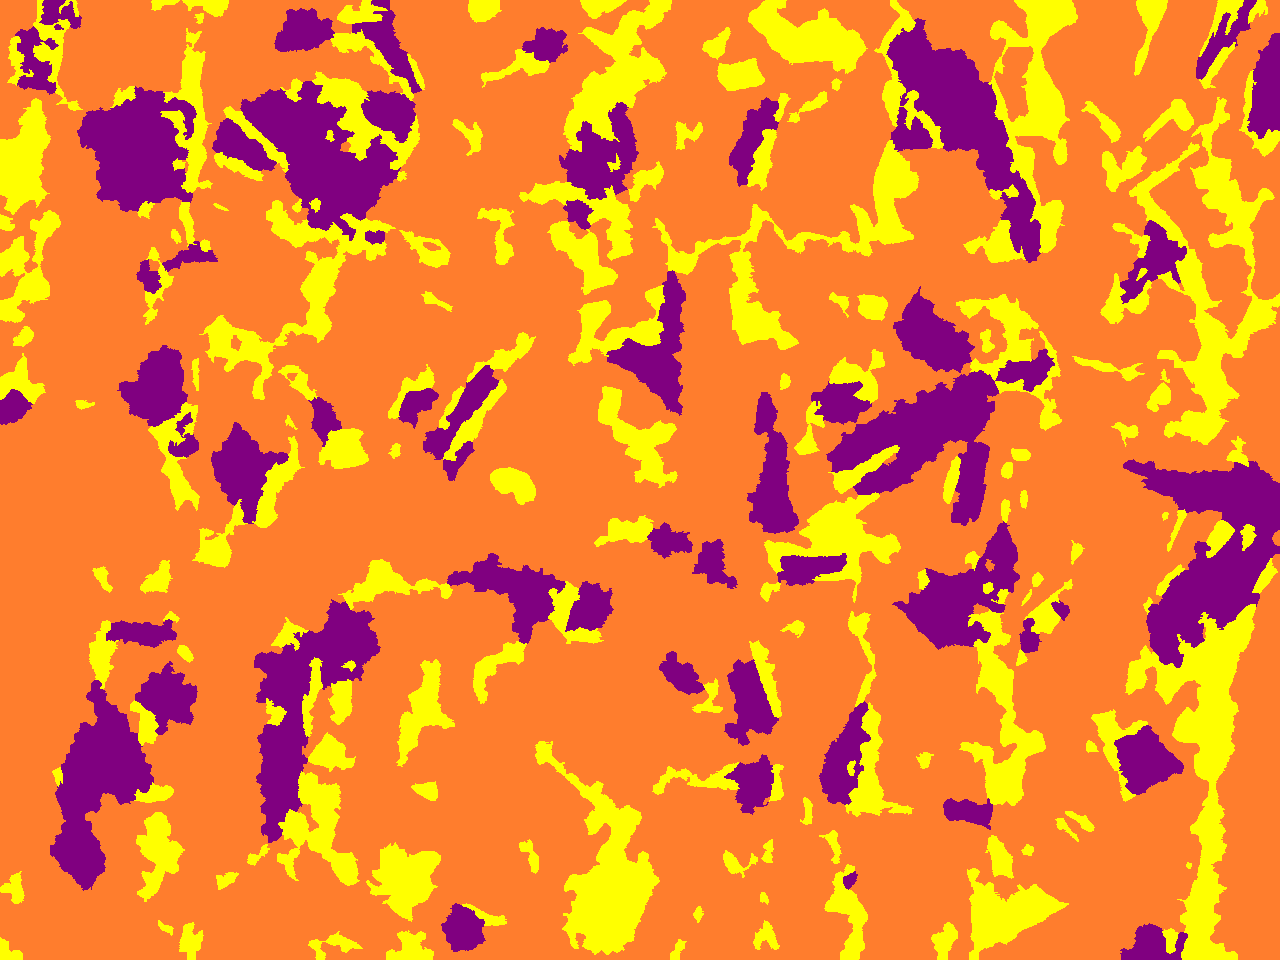
\includegraphics[width=\textwidth]{images/x3000/1_label.png}
		\caption{x3000 label}
		\label{fig:image2.1.2}
	\end{subfigure}
	\hfill
	\begin{subfigure}[b]{0.2\textwidth}
		\centering
		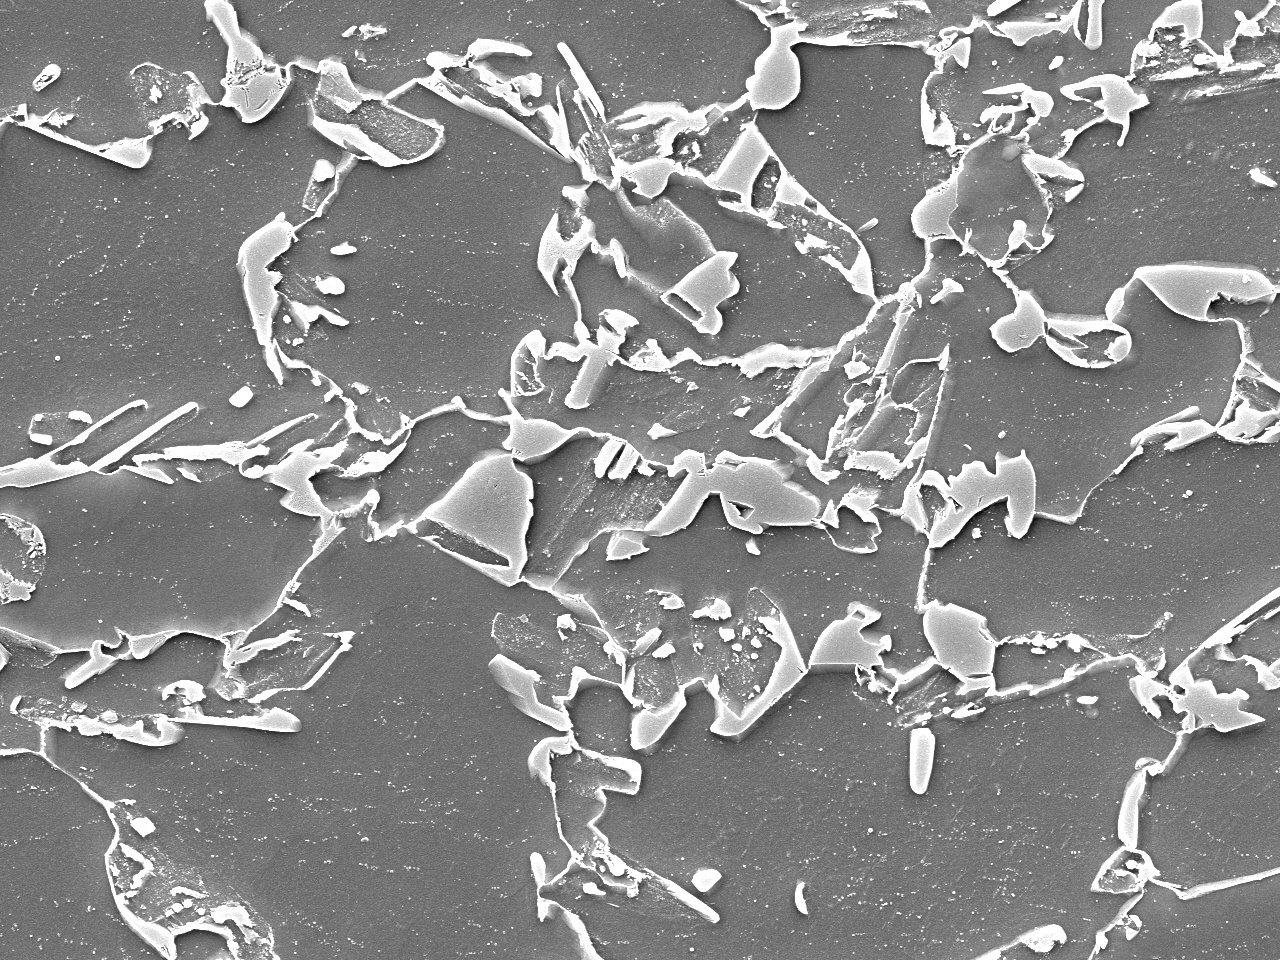
\includegraphics[width=\textwidth]{images/x5000/1.png}
		\caption{x5000 SEM}
		\label{fig:image2.2.1}
	\end{subfigure}
	\begin{subfigure}[b]{0.2\textwidth}
		\centering
		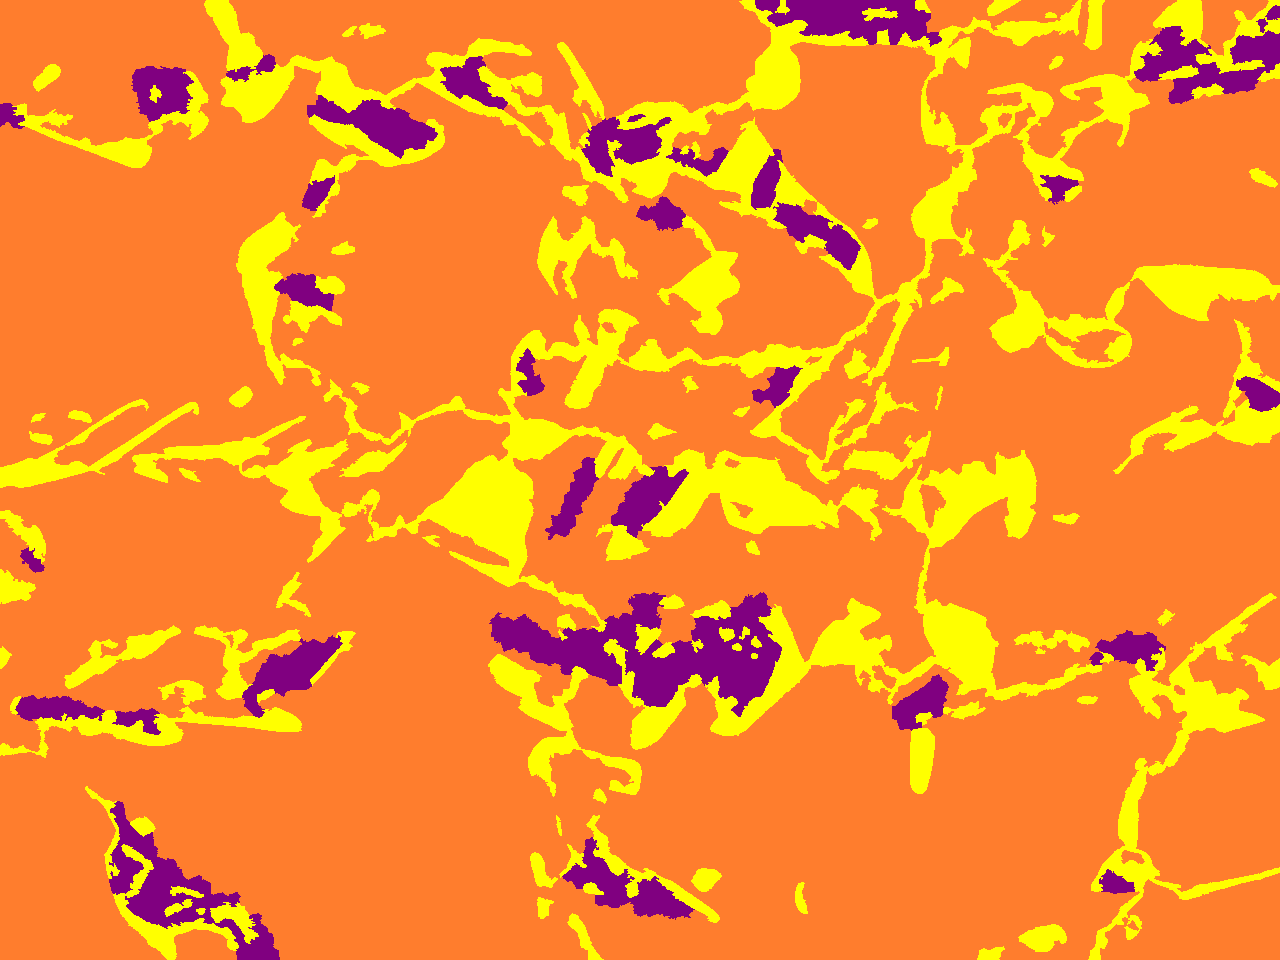
\includegraphics[width=\textwidth]{images/x5000/1_label.png}
		\caption{x5000 label}
		\label{fig:image2.2.2}
	\end{subfigure}
	
	\begin{subfigure}[b]{0.2\textwidth}
		\centering
		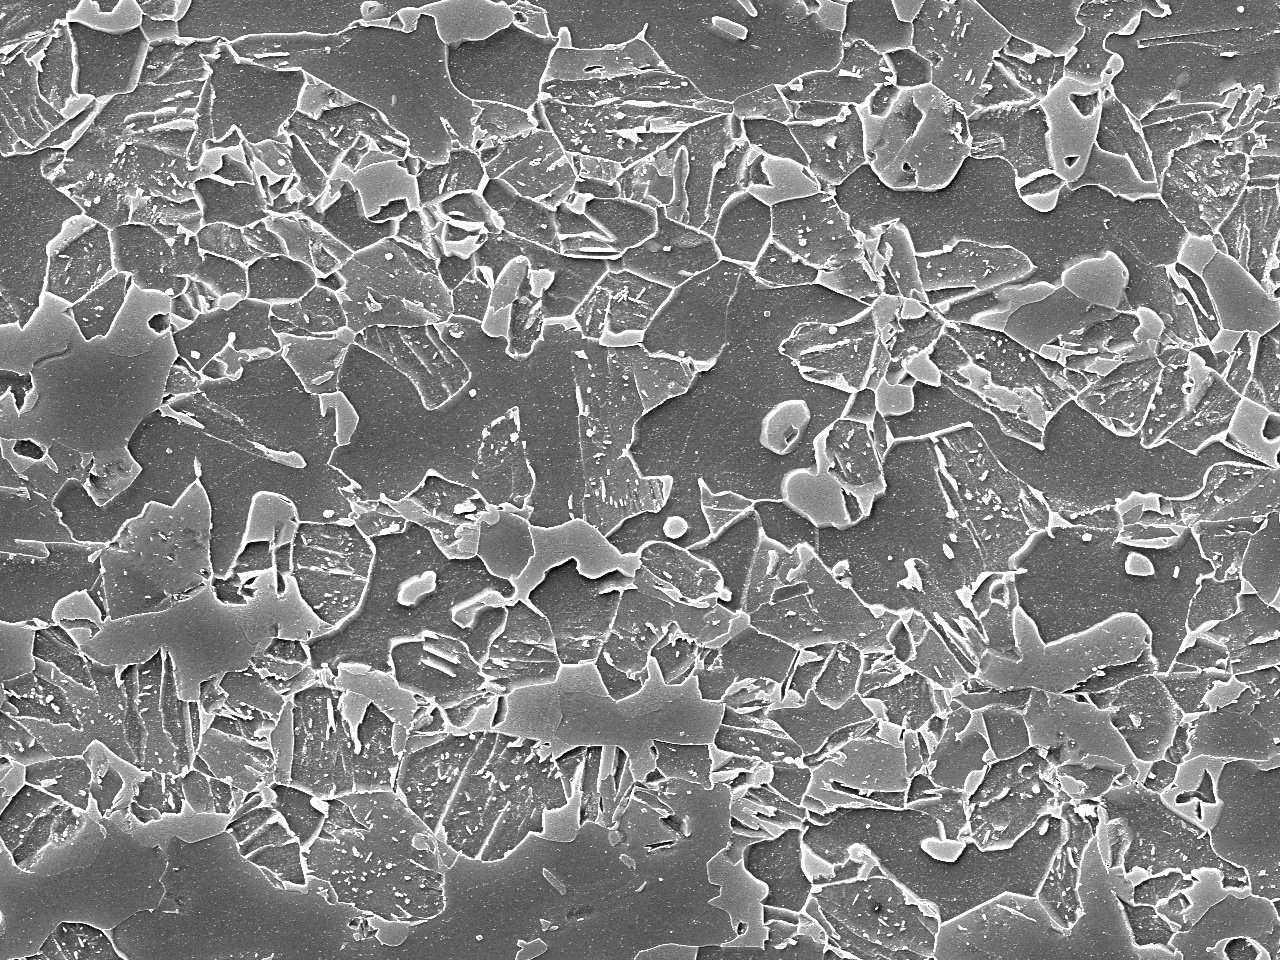
\includegraphics[width=\textwidth]{images/A-type/1.png}
		\caption{A-type SEM}
		\label{fig:image2.3.1}
	\end{subfigure}
	\begin{subfigure}[b]{0.2\textwidth}
		\centering
		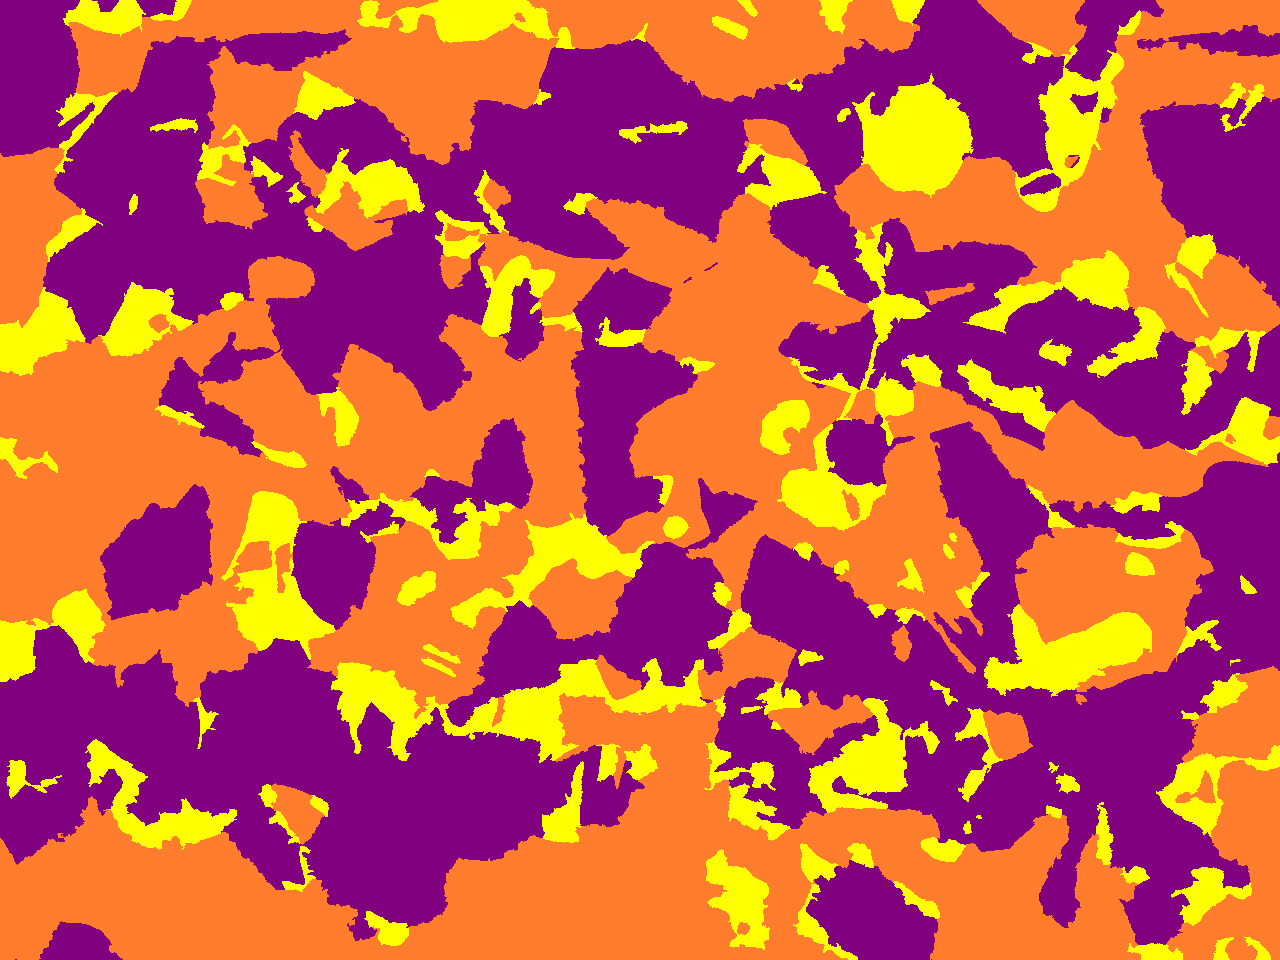
\includegraphics[width=\textwidth]{images/A-type/1_label.png}
		\caption{A-type label}
		\label{fig:image2.3.2}
	\end{subfigure}
	\hfill
	\begin{subfigure}[b]{0.2\textwidth}
		\centering
		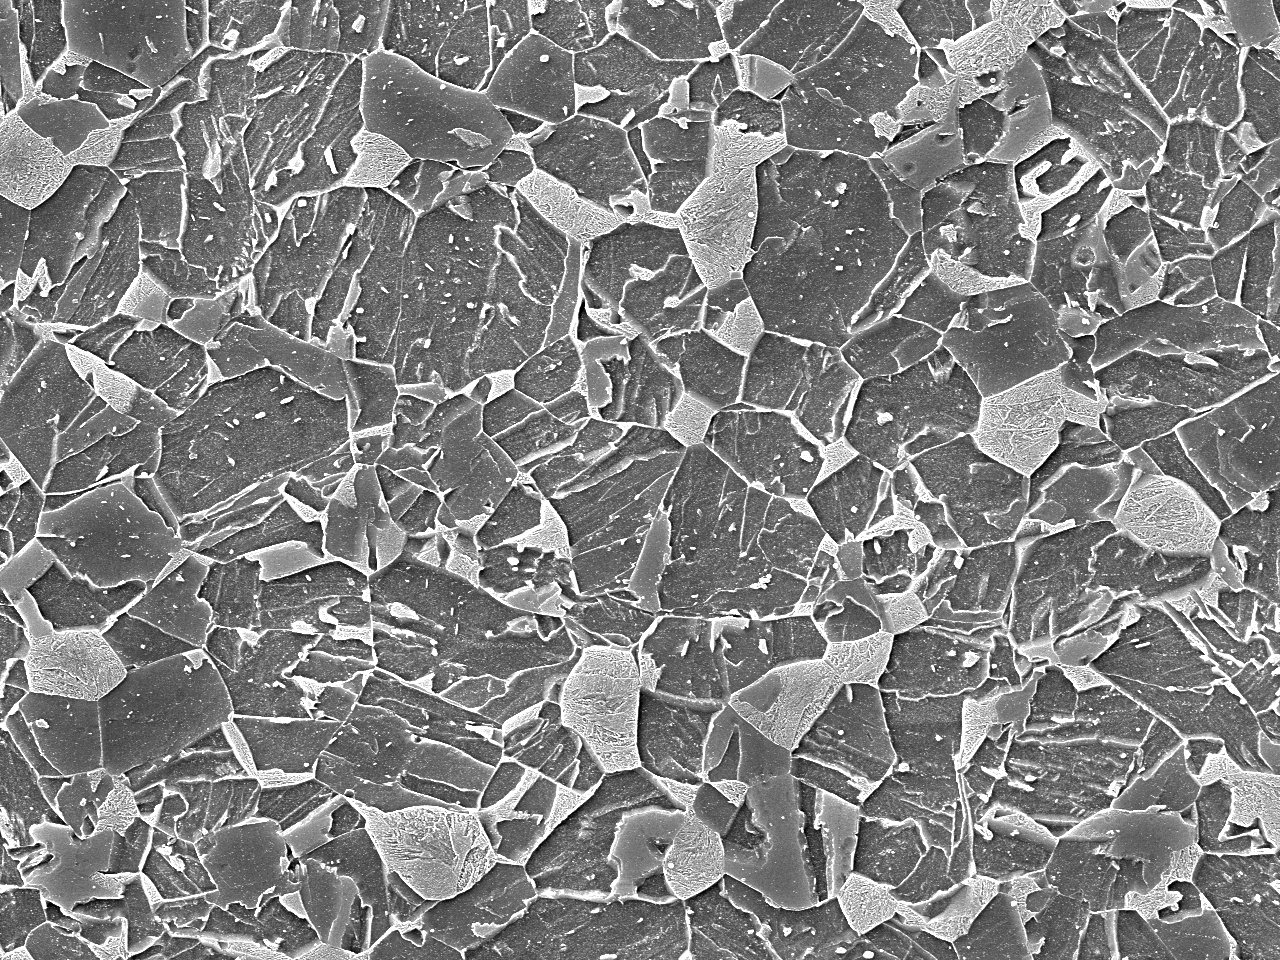
\includegraphics[width=\textwidth]{images/D3-type/1.png}
		\caption{D3-type SEM}
		\label{fig:image2.4.1}
	\end{subfigure}
	\begin{subfigure}[b]{0.2\textwidth}
		\centering
		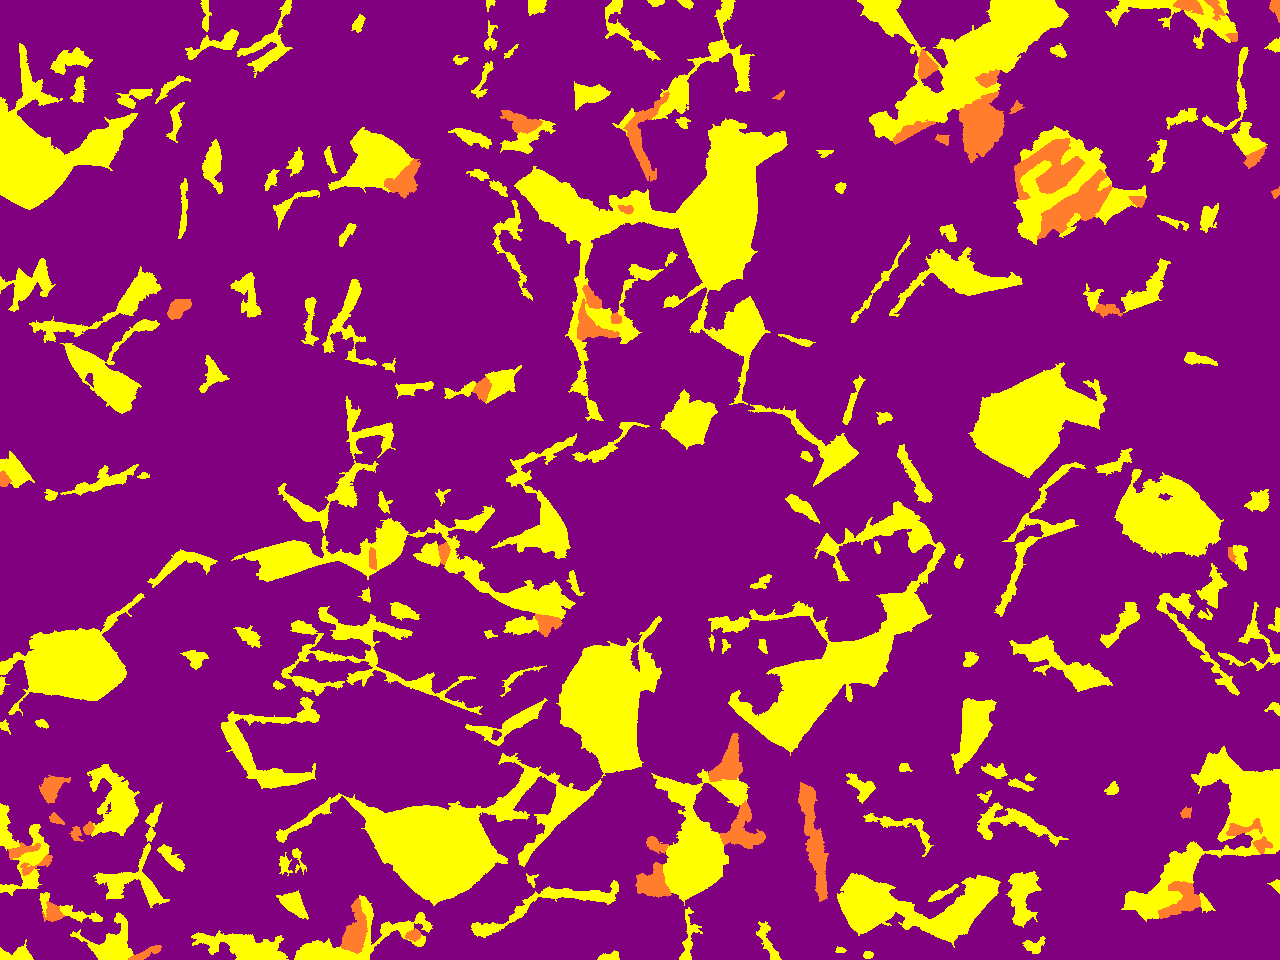
\includegraphics[width=\textwidth]{images/D3-type/1_label.png}
		\caption{D3-type label}
		\label{fig:image2.4.2}
	\end{subfigure}
	
	\begin{subfigure}[b]{0.2\textwidth}
		\centering
		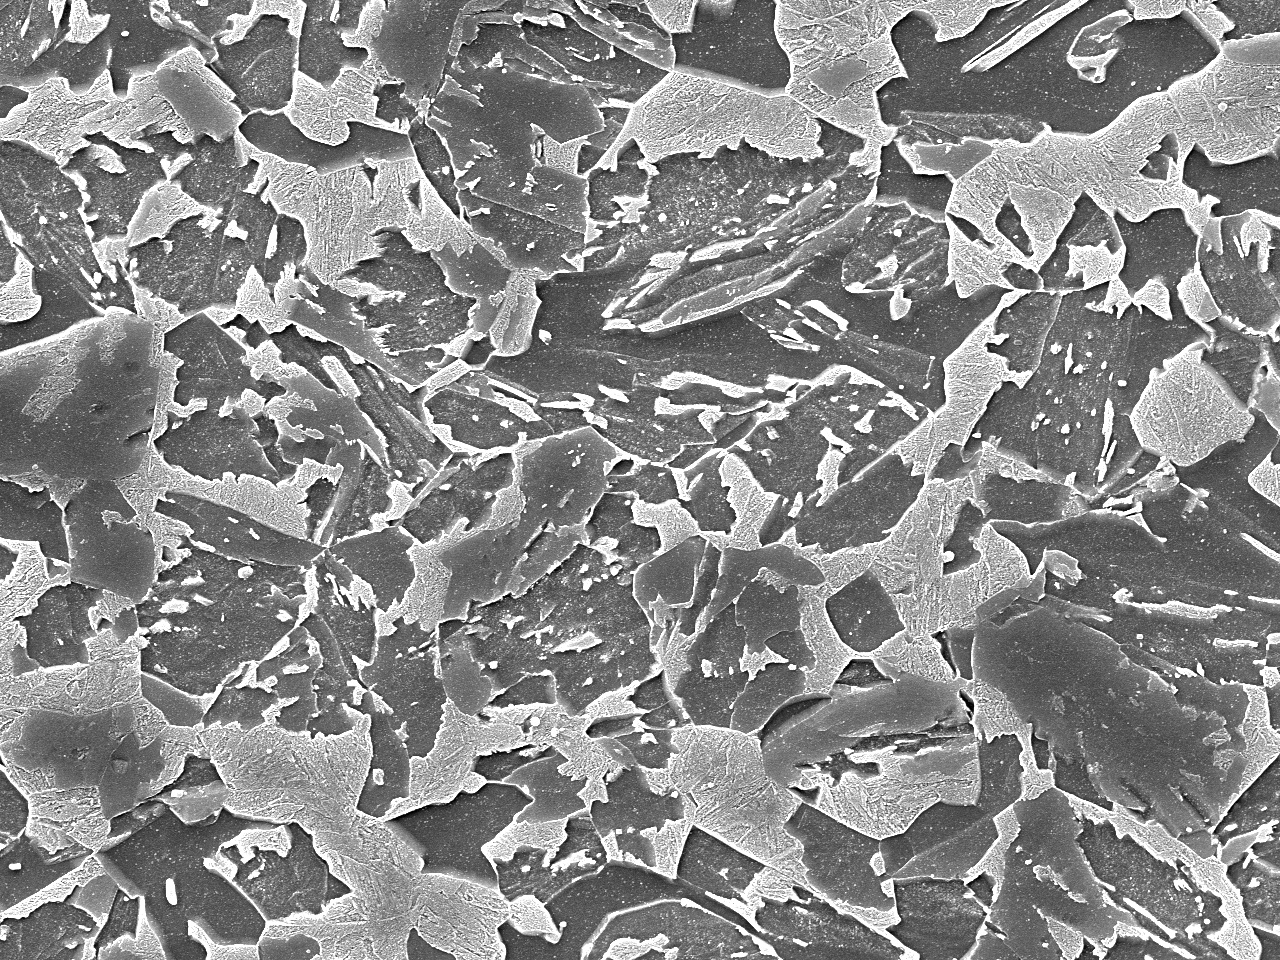
\includegraphics[width=\textwidth]{images/H2-type/1.png}
		\caption{H2-type SEM}
		\label{fig:image2.5.1}
	\end{subfigure}
	\begin{subfigure}[b]{0.2\textwidth}
		\centering
		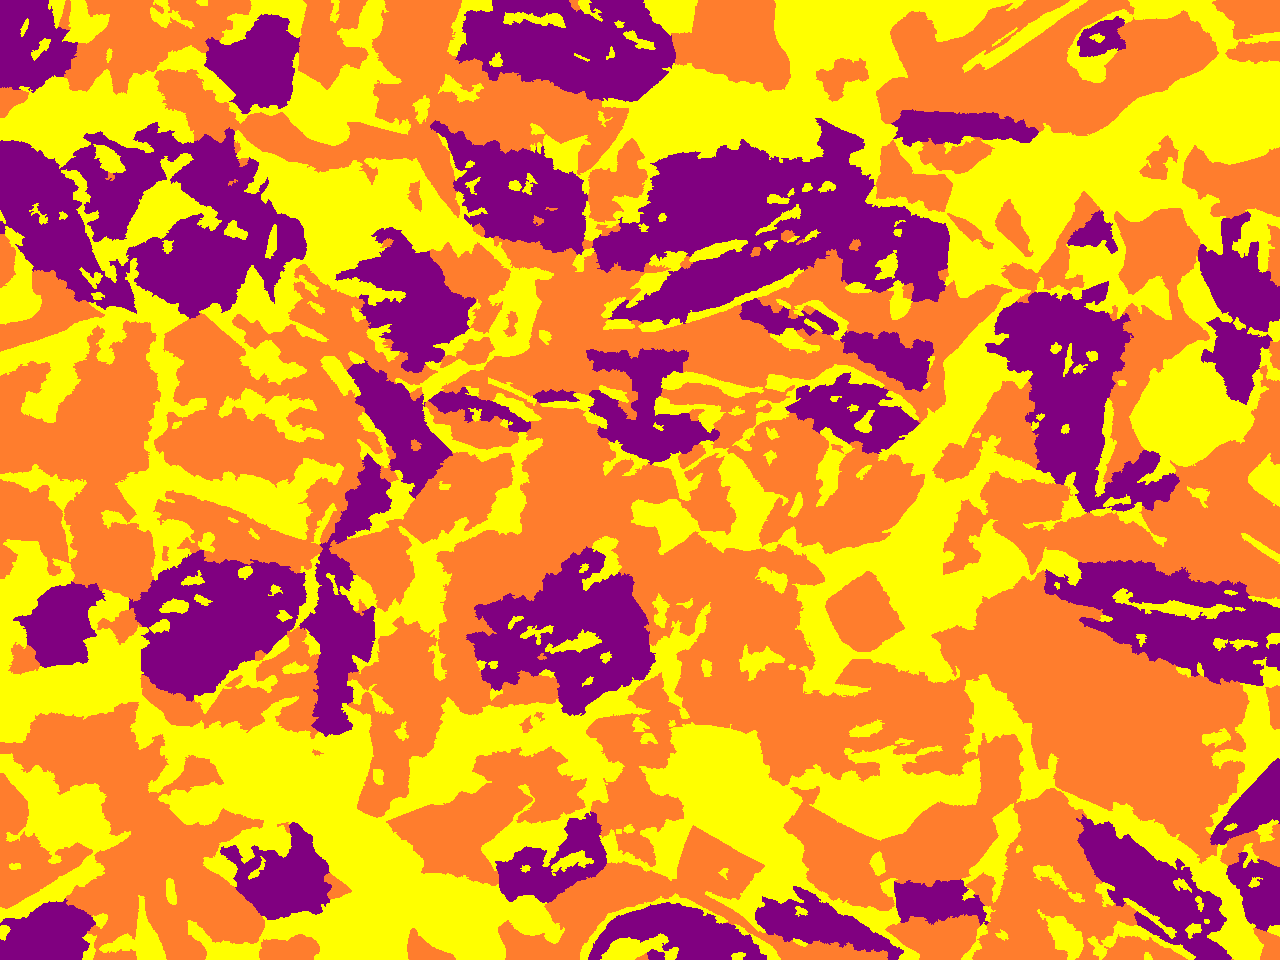
\includegraphics[width=\textwidth]{images/H2-type/1_label.png}
		\caption{H2-type label}
		\label{fig:image2.5.2}
	\end{subfigure}
	\caption{Sample images of various steel and magnification types used during inference.}
	\label{fig:combined}
\end{figure}

It's worth emphasizing that the images magnified at 3000x and 5000x originate from the same E-type steel that was used to train our model. This inclusion demonstrates the model's capacity to effectively scale across varied magnification levels, maintaining its segmentation accuracy even at high magnifications that reveal more intricate microstructures.

Furthermore, the incorporation of A-type, D3-type, and H2-type steel images, all magnified at 5000x, underscores the model's capability to generalize across different steel types. Despite these steel types featuring distinct microstructural characteristics compared to the E-type steel used in training, the model is able to accurately identify and segment their microstructures. This ability to generalize over various steel types suggests the model's potential for broad applicability in real-world industrial contexts, well beyond its initial training data.

\section{Methodology}
In the following section, we detail the methodology employed in our study, specifically designed to tackle the challenges associated with the segmentation of steel microstructures. We conceptualize a deep learning model as comprising four critical components, as depicted in Figure \ref{fig:imageSections}. These components significantly influence the model's output. The first component involves the application of appropriate data augmentations. The second component is the selection of a suitable model architecture. The third component involves the determination of the optimal loss function and activation functions. Lastly, the fourth component involves fine-tuning certain parameters to optimize the model or inclusion of special techniques to address specific issues.

\begin{figure}[ht]
	\centering
	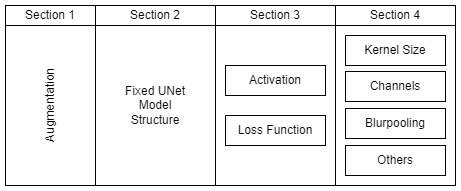
\includegraphics[width=0.7\textwidth]{images/sections.png}
	\caption{The four-step process of modifying the UNet-based model for steel image segmentation. The process includes performing problem-specific augmentations, working with fixed architecture component, optimizing loss and activation functions, and fine-tuning the model.}
	\label{fig:imageSections}
\end{figure}

\subsection{Data Augmentation and Rationale}

Data augmentation techniques serve as essential tools in confronting the issue of data insufficiency by fabricating an expanded training set through various transformations and adaptations of existing samples. The augmentations should be carried out based on the requirements of the problem statement. We employed several augmentation techniques which not only enhanced the diversity of our training dataset but also improved our model's ability to generalize. Below we not the augmentations that we used along with its proper rationale.

\begin{itemize}
	\item Flip (x, y): We introduced horizontal (x-axis) and vertical (y-axis) flipping transformations to our images, creating mirror-like variations. This technique is beneficial as it accounts for varied orientations of steel structures, thereby ensuring our model learns to detect structures irrespective of their orientation.
	\item Rotation (0-90 degrees): Our augmentation suite includes random rotations of images within a 0 to 90-degree range. Given that steel structures in SEM images can exist in myriad orientations, this technique serves to imbue our model with rotation invariance, enabling better generalization.
	\item Zoom (1-2.5x): We applied random scaling to our images, ranging from 1 to 2.5 times their original size. This technique mimics the varied magnification levels in SEM images, thus preparing the model to handle different scales of steel structures.
	\item Intensity (0-10): We incorporated random intensity fluctuations in our images, introducing variations in brightness and darkness akin to diverse lighting conditions or material properties. This helps the model to better withstand intensity variations within steel images.
	\item Gamma (0-10): Adjusting the gamma value of our images served to enhance or suppress specific intensity levels. Gamma augmentation emulates contrast and brightness changes, thereby training the model to recognize features invariant to these differences.
	\item Contrast (HE): By applying histogram equalization (HE) to enhance image contrast, we redistributed pixel intensities to bolster overall contrast. This proved to be particularly beneficial in highlighting finer details and improving segmentation accuracy in low-contrast areas.
	\item Sliding Window: We incorporated the sliding window technique, dividing the larger input images into smaller patches of size 800x800 pixels with a stride of 15 pixels. Opting for larger patches facilitated the capture of complete structural elements, which would have been potentially obscured in smaller patches.
\end{itemize}

\subsection{Setting the Model Architecture}

The second segment involves selecting an appropriate model for the segmentation task. Given that UNet-based models have consistently outperformed other model architectures, we recommend using a UNet-based model such as UNet++, Unet3+, R2Unet, etc. However, our aim is to adapt the UNet models specifically for the task of steel image segmentation. Therefore, we chose the barebone UNet model and demonstrate how it can be adapted for steel image segmentation. The U-Net architecture, depicted in Fig. 3, is designed as a combination of an encoder path and a decoder path. The encoder path is responsible for extracting contextual information, while the decoder path contributes to precise localization.


\begin{figure}[ht]
	\centering
	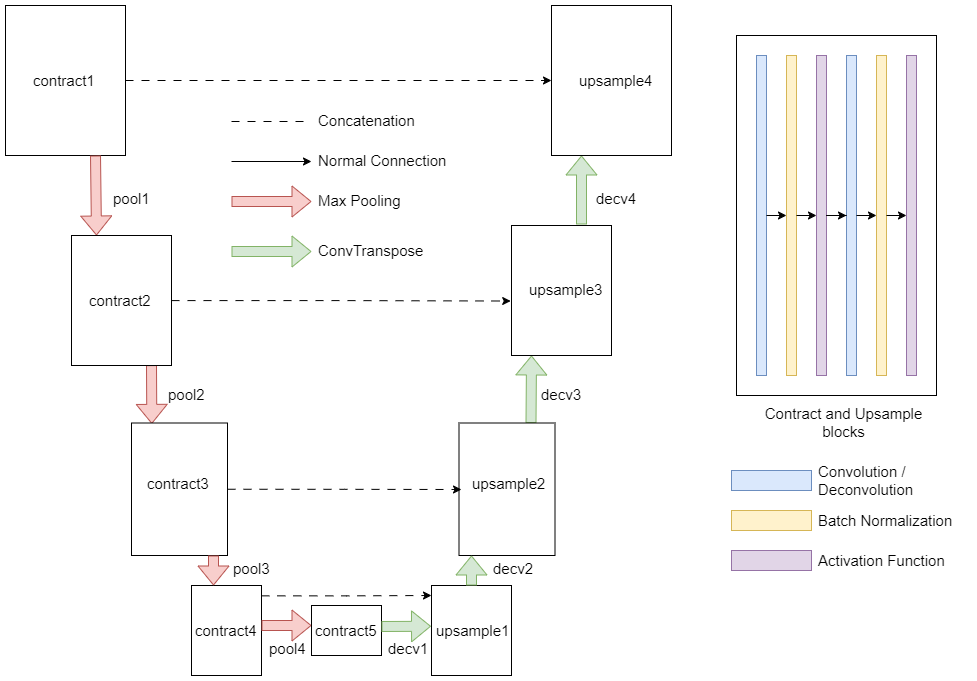
\includegraphics[width=0.8\textwidth]{images/model_updated.png}
	\caption{UNet architecture}
	\label{fig:imageModel}
\end{figure}


The encoder pathway is initiated with a contraction module (contract1), dedicated to applying a series of convolutional operations to discern low-level features from the input image. Subsequent modules, identified as pool1 through pool4, carry out pooling operations that systematically reduce the spatial dimensions of the feature maps, while simultaneously augmenting the number of channels. The subsequent contraction modules, identified as contract2 through contract5, perform additional convolutional operations to distill higher-level features.

Transitioning into the decoder pathway, the architecture aims to restore spatial information and refine the segmentation outcome. The first decoder module, designated as decv1, executes convolution transpose or pixel shuffling operations, hinging on the specified anti-aliasing type. This operation is followed by an up-sampling operation (upsample1) and a concatenation procedure, amalgamating features from the equivalent layer of the encoder path. This process is reiterated through the successive decoder modules, identified as decv2 through decv4, to further enhance the feature refinement.

The final module in the decoder pathway (decv5) applies a convolutional operation to align the extracted features with the desired output classes. The activation functions integrated into the model architecture, such as ReLU, leaky ReLU, and swish, introduce non-linearity, thereby facilitating superior feature representation. 

The U-Net model operates under supervised learning principles. The training process leverages pixel-wise labeled images as the ground truth, optimizing the model to minimize the loss between the predicted segmentation and these labels. By utilizing the U-Net architecture, the proposed model is proficient at capturing the complex details within the microstructure of steel images and accurately segmenting various regions of interest. The synergistic combination of contraction and expansion modules enables the model to learn global contextual information as well as local, fine-grained details, culminating in precise segmentation outcomes.

\subsection{Configuring Loss and Activation functions}

Configuring correct loss and activation functions is paramount to successfully apply a DL model to a given problem. Often times than not these parameters are domain specific, still it is important to find which loss and activation functions work the best. We performed numerous experimentation on finding the suitable loss and activation functions that would suit our specific problem of steel image segmentation.

\subsubsection{Loss Function}
Considering the unique challenges of steel image segmentation that we wanted to address, we propose a new Loss function for our study, SteelSegLoss which is combination of Focal Loss, Jaccard Loss, and Multi-Scale Structural Similarity (MS-SSIM) Loss. Such a combination of losses have never been tried before to the best of our knowledge.
\begin{itemize}
	\item Focal Loss: This loss function is designed to address class imbalance by down-weighting inliers (easy examples) and focusing on outliers (hard examples). In our case, this is particularly useful as certain phases or structures like Bainite were underrepresented in the dataset. By focusing on these challenging examples, the model is encouraged to learn features that distinguish these rare classes, thereby improving the overall segmentation performance.
	\item Jaccard Loss: Also known as Intersection over Union (IoU) loss, it measures the overlap between the predicted segmentation and the ground truth. This loss function is particularly useful for segmentation tasks as it directly optimizes for the quantity we are interested in - the quality of the segmentation. In our case, Jaccard Loss helps the model to accurately capture the boundaries of different phases and structures, which is crucial for determining material properties.
	\item MS-SSIM Loss: The MS-SSIM loss function measures the structural similarity between the predicted and ground truth images. It is designed to capture the texture and structural information in an image. This is particularly useful in steel image segmentation where different phases and structures have distinct textures and shapes. By optimizing the MS-SSIM loss, the model learns to capture these texture and structural differences, thereby improving the segmentation of different phases and structures in the steel microstructures.
\end{itemize}

By combining these three loss functions, the model is encouraged to learn to segment the steel images accurately, taking into account the class imbalance, the need for accurate boundary delineation, and the importance of capturing texture and structural differences.

\subsubsection{Activation Function}

The activation function plays a pivotal role in introducing non-linearity into the learning process. This non-linearity enables the model to learn from the complex patterns and features in the images, which is essential for tasks like ours where the model needs to differentiate between subtle differences in textures and structures. We selected ReLU as the ideal activation function for our task. Although we experimented with LeakyReLU and Swish, they did not perform as well. This could be due to the nature of the steel image segmentation task. ReLU introduces non-linearity without affecting the receptive fields of the convolution layer, which could be beneficial in our task where preserving spatial information (like texture and structure) is crucial. On the other hand, Leaky ReLU and Swish, despite being improvements over ReLU in certain tasks, might not be well-suited for our specific task of steel image segmentation. We also experimented with the SIREN (SINusoidal REpresentation Networks) activation function, which is designed to represent complex natural signals, but it did not perform well in our task.

\subsection{Optimizing Other Parameters and Experimental Techniques}
The final part of the process involves fine-tuning the model. This includes making minor adjustments to the model architecture and hyperparameters to improve performance. We employed the Adam optimizer, renowned for its adaptive learning rate efficiency. We selected a batch size of 16 and channel size of 16, which proved optimal for balancing memory utilization and training efficiency. The learning rate, set at 0.00001, ensured small step sizes for smoother convergence during training. This value was carefully chosen after a series of experiments and fine-tuning to achieve optimal performance
\begin{itemize}
	\item Input size: The input size of the image significantly impacts the performance of the model, especially in tasks like image segmentation where the goal is to capture intricate details and structures in the image. The larger input size allows the model to have more contextual information, improved learning of spatial hierarchies and better handling of variability. Therefore we used an input size of 800x800 and it performed better than 256x256 and 512x512 as expected. It is to be noted that increasing input size also increases the computational cost and memory requirements of the model.
	\item Kernel size: The kernel size in a convolutional layer determines the field of view that the model has when processing the input image and impacts the model's ability to capture relevant features. A smaller kernel size, such as 3x3, means that the model is looking at a smaller portion of the image at a time. This can be beneficial for tasks where the important features are small and localized. A larger kernel size, like 7x7, allows the model to view a larger portion of the image at once, which is beneficial for tasks where important features span across a larger area, as in the structures of the microstructures of steel SEM images. 
	\item Experimental techniques: other features can be added or experimented with for better performance.
	\begin{itemize}
		\item Blurpooling: To further optimize our model, we integrated blur pooling layers into the architecture and tested three variations: up, down, and both up and down. Blur pooling aids in reducing the spatial resolution of feature maps while preserving critical information, potentially enabling the model to identify larger-scale patterns and mitigate overfitting \cite{blurPooling}.
		\item Adding boundary class: We attempted to add a boundary class to the labels by delineating edges between classes. This approach aimed to enhance the model's ability to accurately segment the boundaries of steel structures, a critical element in proper classification and analysis.
	\end{itemize}
	Despite the potential advantages, our experiments with blur pooling layers and the boundary class addition did not yield significant improvements in the model's performance.
\end{itemize}

\section{Experimentation}
\subsection{Evaluation Metrics}

To assess the robustness and accuracy of the proposed model, four primary metrics were used: Mean Pixel Accuracy, Dice Score, Class-wise Accuracy, and Class Distribution Ratio.

\begin{itemize}
	\item \textbf{Mean Pixel Accuracy (MPA):} This metric evaluates the pixel-level accuracy of predictions. The formula for calculating Mean Pixel Accuracy is given as:
	
	\[ MPA = \frac{1}{n_{cl}} \sum_{i} \frac{n_{ii}}{t_i} \]
	
	Here, $n_{ij}$ is the number of pixels of class $i$ predicted as class $j$, $n_{cl}$ is the total number of different classes, and $t_{i}$ is the sum of all pixels of class $i$ ($t_{i} = \sum_{j} n_{ij}$).
	
	\item \textbf{Dice Score (F1 Score):} The Dice Score computes the overlap between the predicted segmentation mask (A) and the ground truth mask (B). The formula is:
	
	\[ Dice = \frac{2 |A \cap B|}{|A| + |B|} \]
	
	Here, $A$ is the predicted segmentation mask, $B$ is the ground truth mask, $|A|$ is the number of pixels in $A$, $|B|$ is the number of pixels in $B$, $|A \cap B|$ calculates the intersection of $A$ and $B$.
	
	\item \textbf{Class-wise Accuracy:} This metric measures the accuracy of model's predictions for each individual class, providing a detailed understanding of its performance across different classes.
	
	\item \textbf{Class Distribution Ratio:} This metric compares the distribution of classes in the predicted segmentation masks with the distribution in the ground truth labels, to identify any potential biases or imbalances in the model's predictions.
\end{itemize}

These metrics holistically measure the performance of the proposed model, reflecting its ability to accurately segment various microstructures, and its generalization across different classes. Utilizing these metrics ensures a balanced and comprehensive evaluation of the model's effectiveness in predicting steel microstructures, providing a well-rounded understanding of its performance.

\subsection{Experiment Setup}

Our model's experimental setup is designed to train and evaluate the model using a combination of different steel images and testing methodologies. The setup uses a high-performance computing system equipped with an NVIDIA A6000 GPU, Intel i7 6700 CPU, running on the Ubuntu 22.10 operating system, and utilizing the PyTorch framework.

\begin{itemize}
	\item \textbf{Data Preparation:} To create an effective training dataset, five out of six available images were chosen for augmentation. The remaining image was reserved solely for testing. This strategy provided a sufficient amount of data for training while also ensuring an independent dataset for testing the model's generalization performance. The color-coding of the label images was converted into class labels: purple (Bainite) was denoted as 0, orange (Ferrite) as 1, and yellow (Martensite) as 2.
	
	\item \textbf{Training and Validation Split:} The augmented dataset was further partitioned into a training set and a validation set with a split ratio of 0.8. This meant 80\% of the augmented images were used for model training, while the remaining 20\% were used for validation. This approach facilitated performance monitoring and model fine-tuning during the training process.
	
	\item \textbf{Model Testing:} Post-training, the model was tested on an image not used during the training or augmentation process. This unseen data served to evaluate the model's capacity to generalize and accurately segment the steel structures. Additionally, X3000, x5000, A, H2, D3 steel type images were inferenced using the saved model post-training.
\end{itemize}


\subsection{Experimental Results}

In this section, we describe the results obtained from the experimental setup. We categorize the inference scenarios into three main categories: inferencing with the same steel type and magnification as the trained model, inferencing with the same steel type but different magnification levels, and inferencing with different steel types and different magnification levels compared to the trained model. 

\subsubsection{Comparison of Stock UNet and Augmentations}

In this subsection, we present a tabular analysis of the performance of various UNet variants on the task of steel image segmentation. We investigate three distinct configurations: the Stock UNet Model with Random Augmentation (RA), the Stock UNet Model with our Custom Augmentation (CA), and the Modified UNet with custom augmentation. Random augmentation includes operations like random flips, rotations, scaling, and brightness adjustments during training.


\begin{table}[h!]
	\centering
	\begin{tabular}{|c|c|c|c|c|c|}
		\hline
		Variations & X3000 E Type & X5000 E Type & A Type & D3 Type & H2 Type \\
		\hline
		Stock UNet + RA & 58.85 (0.5743) & 28.82 (0.2768) & 46.29 (0.4601) & 39.9 (0.3842) & 44.48 (0.4292) \\
		Stock UNet + CA & 70.01 (0.6876) & 78.75 (0.7803) & 64.29 (0.6393) & 55.61 (0.5328) & 63.44 (0.6233) \\
		\rowcolor{yellow!30} Mod UNet + CA & 84.11 (0.8389) & 89.29 (0.8892) & 77.78 (0.7731) & 68.32 (0.6809) & 73.92 (0.7376) \\
		\hline
	\end{tabular}
	\caption{Performance Comparison of basic and modified UNet model with our Augmentation Strategies on Steel Image Segmentation Task.}
\end{table}

\subsubsection{Inference on Same Steel and Same Magnification}

The trained model was evaluated using a test image that was isolated from the training process. The model achieved an overall pixel accuracy of 91.74\%, with a dice score of 0.9158 as shown in table 2 and figure 5. The class-wise accuracy analysis showed that the model performed significantly well across different classes: Martensite (83.7\%), Ferrite (96.1\%), and Bainite (81.3\%). 


\begin{figure}[ht]
	\centering
	
	\begin{subfigure}[b]{0.3\textwidth}
		\centering
		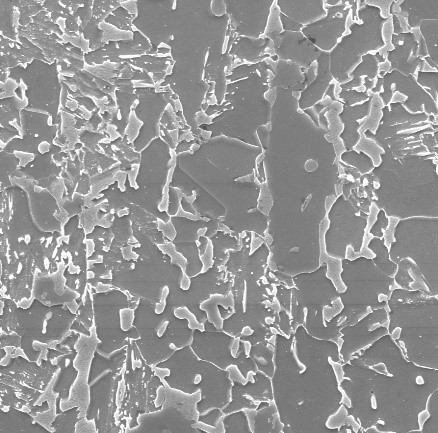
\includegraphics[width=\textwidth]{images/inference/SameSteelSameMag-O.jpg}
		\caption{}
		\label{fig:samesteelsamemag-orig}
	\end{subfigure}
	\hfill
	\begin{subfigure}[b]{0.3\textwidth}
		\centering
		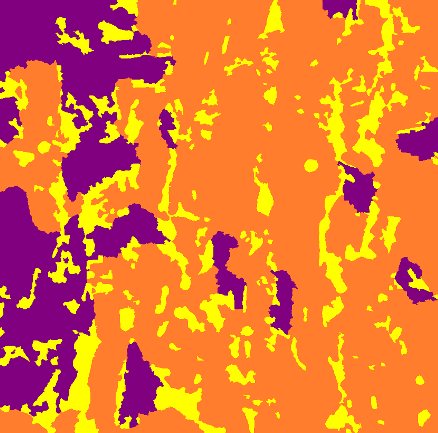
\includegraphics[width=\textwidth]{images/inference/SameSteelSameMag-L.png}
		\caption{}
		\label{fig:samesteelsamemag-label}
	\end{subfigure}
	\hfill
	\begin{subfigure}[b]{0.3\textwidth}
		\centering
		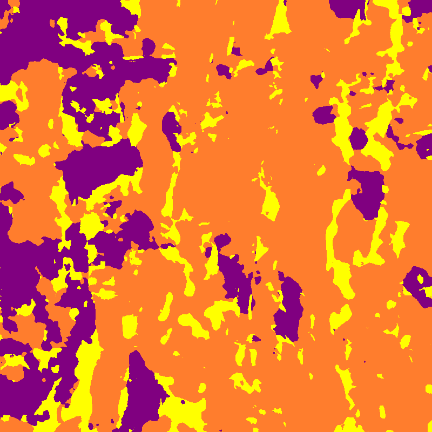
\includegraphics[width=\textwidth]{images/inference/SameSteelSameMag-P.png}
		\caption{}
		\label{fig:samesteelsamemag-pred}
	\end{subfigure}
	
	\caption{(a) x2700 magnified E type SEM test image (b) Corresponding label image by EBSD (c) Image predicted by our model.}
	\label{fig:samesteelsamemag}
\end{figure}



\begin{table}[h!]
	\centering
	\begin{tabular}{|c|c|}
		\hline
		\textbf{Image Type} & \textbf{Test Image Accuracy}\\
		\hline
		Pixel Accuracy & 91.74 (0.9158) \\
		\hline
		Martensite & 83.7 \\
		Ferrite & 96.1 \\
		Bainite & 81.3 \\
		\hline
	\end{tabular}
	\caption{Accuracy and Dice measurements of test image}
\end{table}

\subsubsection{Inference on Same Steel with Different Magnification}

Images of the same Steel type (E type) but at different magnification levels were used for inference. Images at x3000 and x5000 zoom levels were used, revealing accuracies of 84.11\% and 89.3\%, respectively as shown in table 3 and figure 6. The additional evaluation metrics, including the Dice score, accuracy per class, and class ratio, provided a deeper understanding of the model performance across different magnification levels. 
\begin{figure}[ht]
	\centering
	
	\begin{subfigure}[b]{0.3\textwidth}
		\centering
		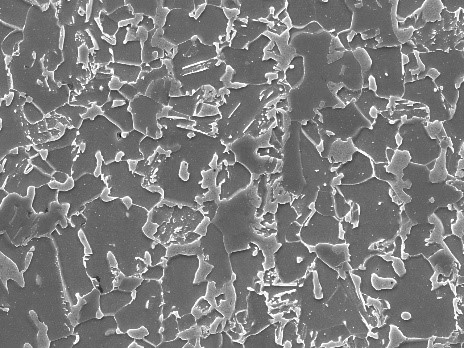
\includegraphics[width=\textwidth]{images/inference/SameSteelDiffMag-O.jpg}
		\caption{}
		\label{fig:samesteeldiffmag3K-orig}
	\end{subfigure}
	\hfill
	\begin{subfigure}[b]{0.3\textwidth}
		\centering
		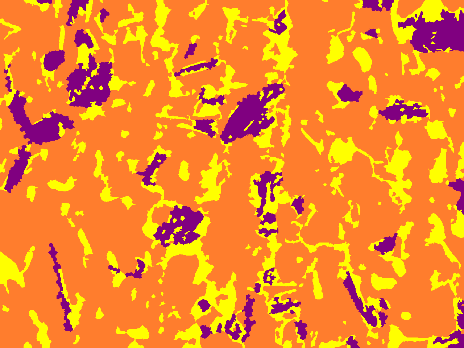
\includegraphics[width=\textwidth]{images/inference/SameSteelDiffMag-L.png}
		\caption{}
		\label{fig:samesteeldiffmag3K-label}
	\end{subfigure}
	\hfill
	\begin{subfigure}[b]{0.3\textwidth}
		\centering
		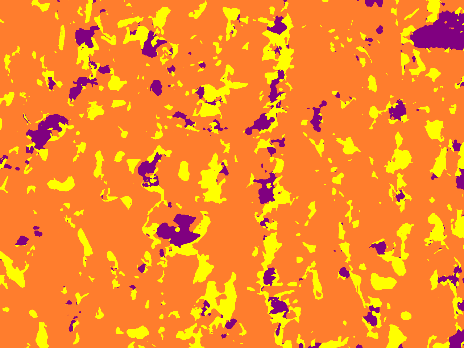
\includegraphics[width=\textwidth]{images/inference/SameSteelDiffMag-P.png}
		\caption{}
		\label{fig:samesteeldiffmag3K-pred}
	\end{subfigure}
		\begin{subfigure}[b]{0.3\textwidth}
		\centering
		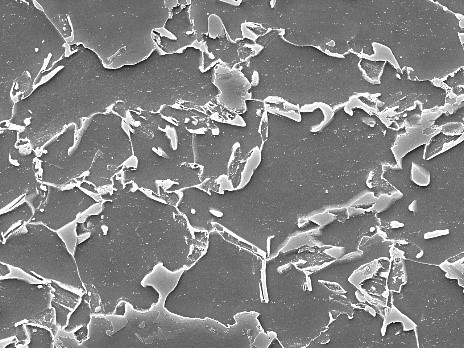
\includegraphics[width=\textwidth]{images/inference/SameSteelDiffMag-2-O.jpg}
		\caption{}
		\label{fig:samesteeldiffmag5K-orig}
	\end{subfigure}
	\hfill
	\begin{subfigure}[b]{0.3\textwidth}
		\centering
		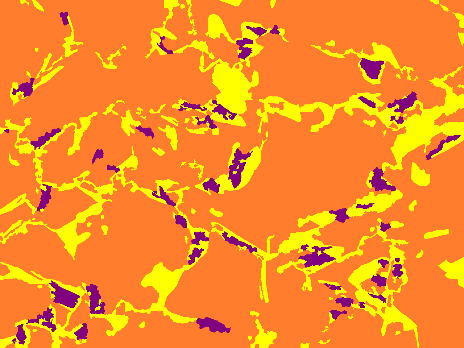
\includegraphics[width=\textwidth]{images/inference/SameSteelDiffMag-2-L.png}
		\caption{}
		\label{fig:samesteeldiffmag5K-label}
	\end{subfigure}
	\hfill
	\begin{subfigure}[b]{0.3\textwidth}
		\centering
		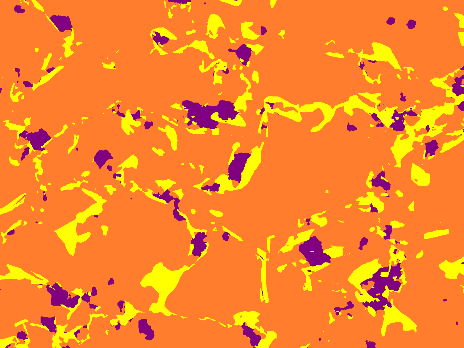
\includegraphics[width=\textwidth]{images/inference/SameSteelDiffMag-2-P.png}
		\caption{}
		\label{fig:samesteeldiffmag5K-pred}
	\end{subfigure}
	
	\caption{(a), (b) x3000 magnified E type SEM test image and corresponding label; (d), (e) x5000 magnified E type SEM test image and corresponding label; (c), (f) Images predicted by our model.}
	\label{fig:samesteeldiffmag}
\end{figure}


\begin{table}[h!]
	\centering
	\begin{tabular}{|c|c|c|}
		\hline
		\textbf{Metrics} & \textbf{X3000 E Type} & \textbf{X5000 E Type}\\
		\hline
		Pixel Accuracy & 84.11 & 89.29 \\
		\hline
		Dice Score & 0.8389 & 0.8892 \\
		\hline
		Accuracy Per Class & 68.11, 93.77, 45.33 & 70.87, 96.57, 41.73 \\
		\hline
		Class Ratio [label] & 0.1982, 0.7029, 0.0989 & 0.176, 0.7789, 0.0451 \\
		\hline
		Class Ratio [Predicted] & 0.1514, 0.7904, 0.0583 & 0.1282, 0.8196, 0.0522 \\
		\hline
		Error Margin of Class Ratio & -0.0438, +0.0875, -0.0406 & -0.0478, +0.0407, +0.0071 \\
		\hline
	\end{tabular}
	\caption{Different metrics of predicted images of x3000 and x5000 E type steel}
\end{table}

\subsubsection{Inference on Different Steel and Different Magnification}

The performance of the model was further assessed on images of different steel types and magnification levels not included in the training data. The model demonstrated decent accuracies on these images, with A type steel images achieving 74.78\%, D3 type achieving 68.3\%, and H2 type achieving nearly 74\% as shown in table 4 and can be visualized in figure 7. 


\begin{figure}[!h]
	\centering
	
	\begin{subfigure}[b]{0.3\textwidth}
		\centering
		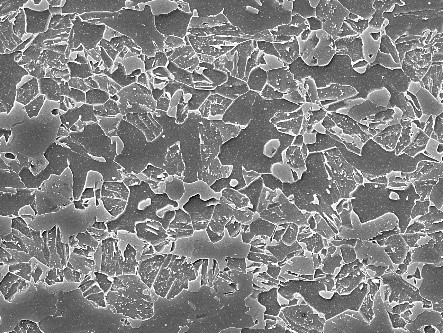
\includegraphics[width=\textwidth]{images/inference/A-type-O.jpg}
		\caption{}
		\label{fig:A-type-orig}
	\end{subfigure}
	\hfill
	\begin{subfigure}[b]{0.3\textwidth}
		\centering
		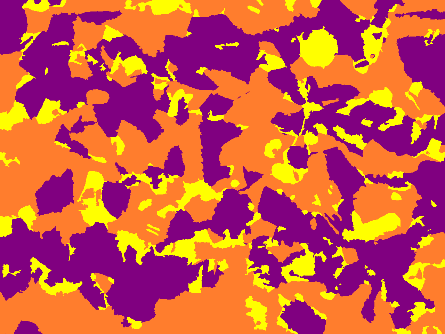
\includegraphics[width=\textwidth]{images/inference/A-type-L.png}
		\caption{}
		\label{fig:A-type-label}
	\end{subfigure}
	\hfill
	\begin{subfigure}[b]{0.3\textwidth}
		\centering
		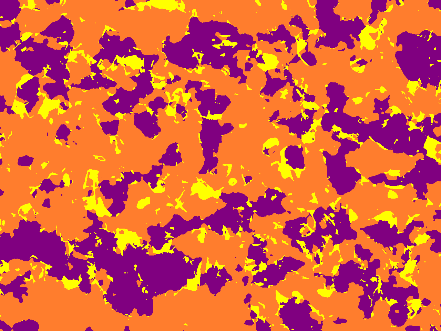
\includegraphics[width=\textwidth]{images/inference/A-type-P.png}
		\caption{}
		\label{fig:A-type-pred}
	\end{subfigure}
	\begin{subfigure}[b]{0.3\textwidth}
		\centering
		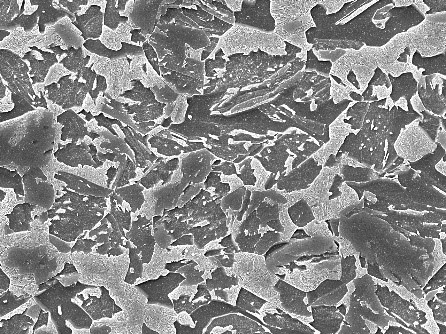
\includegraphics[width=\textwidth]{images/inference/H2-type-O.jpg}
		\caption{}
		\label{fig:H2-type-orig}
	\end{subfigure}
	\hfill
	\begin{subfigure}[b]{0.3\textwidth}
		\centering
		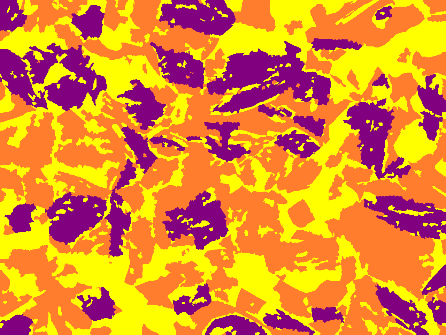
\includegraphics[width=\textwidth]{images/inference/H2-type-L.png}
		\caption{}
		\label{fig:H2-type-label}
	\end{subfigure}
	\hfill
	\begin{subfigure}[b]{0.3\textwidth}
		\centering
		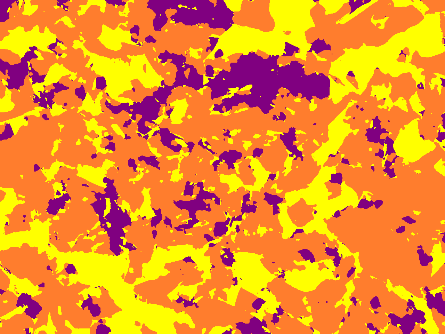
\includegraphics[width=\textwidth]{images/inference/H2-type-P.png}
		\caption{}
		\label{fig:H2-type-pred}
	\end{subfigure}
	\begin{subfigure}[b]{0.3\textwidth}
		\centering
		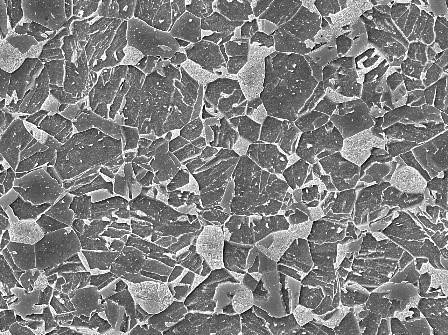
\includegraphics[width=\textwidth]{images/inference/D3-type-O.jpg}
		\caption{}
		\label{fig:D3-type-orig}
	\end{subfigure}
	\hfill
	\begin{subfigure}[b]{0.3\textwidth}
		\centering
		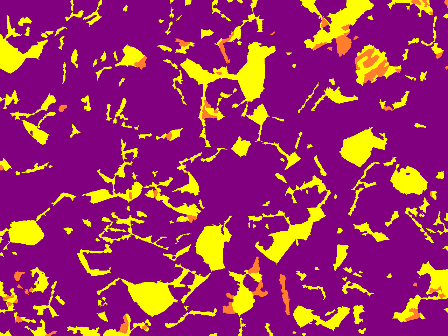
\includegraphics[width=\textwidth]{images/inference/D3-type-L.png}
		\caption{}
		\label{fig:D3-type-label}
	\end{subfigure}
	\hfill
	\begin{subfigure}[b]{0.3\textwidth}
		\centering
		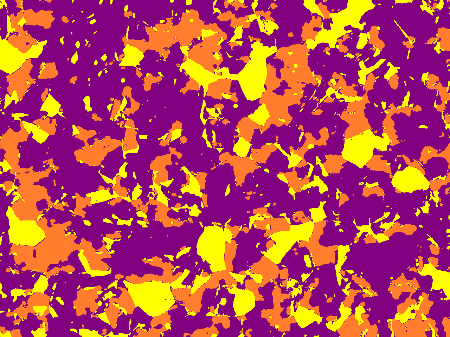
\includegraphics[width=\textwidth]{images/inference/D3-type-P.png}
		\caption{}
		\label{fig:D3-type-pred}
	\end{subfigure}
	
	\caption{(a), (b) x5000 magnified A type SEM test image and corresponding label; (d), (e) x5000 magnified D3 type SEM test image and corresponding label; (g), (h) x5000 magnified H2 type SEM test image and corresponding label; (c), (f) and(i) Images predicted by our model.}
	\label{fig:diffsteeldiffmag}
\end{figure}


\begin{table}[h!]
	\centering
	\begin{tabular}{|c|c|c|c|}
		\hline
		\textbf{Metrics} & \textbf{A type} & \textbf{D3 Type} & \textbf{H2 Type}\\
		\hline
		Pixel Accuracy & 77.78 & 68.32 & 73.92 \\
		\hline
		Dice Score & 0.7731 & 0.6909 & 0.7376 \\
		\hline
		Accuracy Per Class & 51.04, 92.11, 65.45 & 79.64, 24.41, 66.89 & 78.52, 88.11, 37.62 \\
		\hline
		Class Ratio [label] & 0.1441, 0.4281, 0.4278 & 0.1742, 0.0184, 0.8074 & 0.3404, 0.4313, 0.2283 \\
		\hline
		Class Ratio [Predicted] & 0.1, 0.5683, 0.3317 & 0.1796, 0.236, 0.5844 & 0.2819, 0.573, 0.1451 \\
		\hline
		Error Margin of Class Ratio & -0.0441, 0.1402, -0.0961 & 0.0054, 0.2176, -0.223 & -0.0585, 0.1417, -0.0832 \\
		\hline
	\end{tabular}
	\caption{Different metrics of predicted images of different types of steel}
\end{table}

\subsubsection{Comparison on Other Datasets}

To further validate the effectiveness of our proposed method, we compared its performance with other established models, namely PixelNet, UNet, and UNet++, on two different datasets: UHCS and MetalDAM. The results of this comparison are presented in Table 1 and as shown in the table, our proposed method outperforms the other models on both datasets.

\begin{table}[h!]
	\centering
	\begin{tabular}{|c|c|c|c|c|}
		\hline
		\textbf{Dataset} & \textbf{PixelNet} & \textbf{UNet} & \textbf{UNet++} & \textbf{Our Proposal} \\
		\hline
		UHCS & 90.77 & 91.15 & 91.15 & \textbf{95.79}\\
		\hline
		MetalDAM & 84.07 & 86.33 & 87.04 & \textbf{94.21}\\
		\hline
	\end{tabular}
	\caption{Performance comparison of PixelNet, UNet, UNet++, and our proposed method on UHCS and MetalDAM datasets.}
\end{table} 



\subsection{Ablation Studies}

\subsubsection{Activation Function}
Different activation functions were examined to determine their impact on the model performance. ReLU performed better as illustrated in Table 5.

\begin{table}[h!]
	\centering
	\begin{tabular}{|c|c|c|c|c|c|}
		\hline
		Activation & X3000 E Type & X5000 E Type & A Type & D3 Type & H2 Type \\
		\hline
		Siren & 86.12 (0.8487) & 89.77 (0.8853) & 74.87 (0.7383) & 40.02 (0.3994) & 69.8 (0.6855) \\
		\rowcolor{yellow!30} ReLU & 84.11 (0.8389) & 89.29 (0.8892) & 77.78 (0.7731) & 68.32 (0.6809) & 73.92 (0.7376) \\
		Leaky ReLU & 84.77 (0.8452) & 88.53 (0.8831) & 75.19 (0.7493) & 59.59 (0.5855) & 69.69 (0.6938) \\
		Swish & 84.21 (0.8396) & 88.67 (0.8842) & 72.41 (0.7217) & 56.54 (0.5649) & 70.00 (0.6973) \\
		\hline
	\end{tabular}
	\caption{Pixel Accuracy and dice measurements along with class-wise accuracy for models with different activation functions.}
\end{table}

\subsubsection{Effects of Blur Pooling}
Blur pooling layers were tested in different combinations to analyze their impact on model performance in Table 6. As observed, blur pooling did nt make any improvements to the model performance.

\begin{table}[h!]
	\centering
	\begin{tabular}{|c|c|c|c|c|c|}
		\hline
		Blur Pool & X3000 E Type & X5000 E Type & A Type & D3 Type & H2 Type \\
		\hline
		\rowcolor{yellow!30} None & 84.11 (0.8389) & 89.29 (0.8892) & 77.78 (0.7731) & 68.32 (0.6809) & 73.92 (0.7376) \\
		Down & 83.53 (0.8329) & 87.69 (0.8743) & 70.83 (0.7061) & 52.5 (0.5227) & 68.02 (0.6777) \\
		Up & 84.41 (0.8416) & 87.93 (0.8768) & 76.73 (0.7648) & 45.04 (0.4479) & 69.0 (0.6875) \\
		Down + Up & 84.3 (0.8405) & 87.51 (0.8726) & 74.5 (0.7425) & 40.24 (0.3999) & 66.78 (0.6653) \\
		\hline
	\end{tabular}
	\caption{Pixel Accuracy and dice measurements along with class-wise accuracy for models with different Blur pooling layers.}
\end{table}

\subsubsection{Loss Functions}
Model results with different loss functions - Focal Loss, Jaccard Loss and SteelSeg loss is detailed in table 7. 

\begin{table}[h!]
	\centering
	\begin{tabular}{|c|c|c|c|c|c|}
		\hline
		Loss & X3000 E Type & X5000 E Type & A Type & D3 Type & H2 Type \\
		\hline
		Focal & 81.97 (0.7972) & 87.01 (0.8676) & 74.68 (0.7116) & 61.75 (0.5997) & 70.89 (0.6764) \\
		Jaccard & 83.35 (0.8168) & 86.06 (0.8459) & 75.94 (0.7231) & 65.34 (0.6392) & 72.47 (0.7076) \\
		\rowcolor{yellow!30} SteelSegLoss & 84.11 (0.8389) & 89.29 (0.8892) & 77.78 (0.7731) & 68.32 (0.6809) & 73.92 (0.7376) \\
		\hline
	\end{tabular}
	\caption{Pixel Accuracy and dice measurements along with class-wise accuracy for models with different loss functions.}
\end{table}

\subsubsection{Inclusion of Boundary Class}
Introducing a boundary class in the classification task was intended to improve boundary localization, enhancing discrimination, reducing ambiguity, and enabling fine-grained analysis.

\begin{table}[h!]
	\centering
	\begin{tabular}{|c|c|c|c|c|c|}
		\hline
		Class & X3000 E Type & X5000 E Type & A Type & D3 Type & H2 Type \\
		\hline
		\rowcolor{yellow!30} w/o Boundary Class & 84.11 (0.8389) & 89.29 (0.8892) & 77.78 (0.7731) & 68.32 (0.6809) & 73.92 (0.7376) \\
		w Boundary Class & 80.04 (0.7979) & 84.94 (0.8469) & 70.95 (0.707) & 62.53 (0.6228) & 65.02 (0.6477) \\
		\hline
	\end{tabular}
	\caption{Accuracy and dice measurements along with class-wise accuracy for models with boundary class and non-boundary class.}
\end{table}



\section{Discussion}

The experimental results from this study provide valuable insights into the nuances of steel image segmentation. This section provides an analysis and interpretation of these results, addressing the strengths and limitations of our approach, investigating the factors influencing performance variations, discussing the encountered challenges, and outlining potential future work and improvement areas.

\subsection{Experimental Results Analysis and Interpretation}

In this study, we evaluated different aspects of a segmentation model, we performed experiments on multi-phase EBSD images, performed experiments with various configurations keeping a overall fixed UNet structure including activation functions, blur pooling, loss functions, incorporation of boundary class and conducted scalability experimentation on different magnification and steel types. 
Several factors contributed to the observed performance of the model. 

\begin{itemize}
	\item Augmentations of data was a significant aspect of the model performance and it should be carefully performed keeping the objective in sight.
	\item Our proposed SteelSegLoss function focussed on outlier examples and encouraged the model to learn and distinguish rare classes. It not only identified different phases and structures but also different textures and shapes.
	\item Clearly ReLU activation function performed better than SIREN. ReLU activation function outputs a range from 0 to positive infinity. This means that it effectively removes negative values during the forward propagation process, introducing sparsity in the network and thereby helping with reducing overfitting. On the other hand, SIREN oscillates between -1 and 1. This can be beneficial for tasks that require modeling of periodic functions or when the output needs to be normalized to a specific range. However, in the case of a multi-class segmentation task like ours, where the output is a discrete class value, having an output that oscillates between negative and positive values might not be ideal. 
	\item BlurPool layers, also known as anti-aliasing layers, are typically used to reduce high-frequency artifacts in the feature maps. he benefits of BlurPool layers are often most pronounced in tasks where high-frequency noise is a significant issue, such as in certain types of image classification tasks. However, in the case of steel microstructure image segmentation, the primary challenge is not necessarily high-frequency noise, but rather the complex and subtle differences between different phases of the steel. Therefore, the addition of BlurPool layers did not yield favorable results.
	\item The introduction of a boundary class is often used in segmentation tasks to help the model distinguish the transition areas between different classes, especially when the boundaries are not clearly defined. But our experimentation results showed that inclusion of boundary class did not produce expected outcomes.The boundaries between different phases might be highly complex and not easily captured by a simple boundary class. The transitions might involve subtle changes in texture and structure that require more sophisticated modeling approaches.
\end{itemize}
 

\subsection{Challenges and Limitations}

A major challenge encountered in this study is the limited amount of training data. With just six images, the training dataset might not sufficiently capture the diversity and complexity of real-world steel images, potentially affecting the model's generalization capabilities. 

Additionally, there are instances where a microstructure in the steel images may appear similar yet have different compositions. It is important to not only capture texture information but also shape and structure of the microstructures in the image which becomes an inheritantly complex task for the model. Absence of any demarcation between different phases of steel in EBSD also poses another challenge in the segmentation task. 

\section{Conclusion}

This study has presented a comprehensive approach to the segmentation of steel microstructure images, a task of significant importance in the manufacturing industry. We have demonstrated the potential of adapting the UNet architecture, a model originally designed for medical image segmentation, to the specific challenges of steel image segmentation. Our approach has shown that the performance of the model can be significantly improved by carefully selecting and tuning the model parameters, rather than using off-the-shelf configurations.

We have also highlighted the importance of data augmentation in addressing the challenges posed by the intricate and complex nature of steel microstructures. By applying appropriate augmentations, we have been able to enhance the model's ability to capture both the texture and structure of different phases in the microstructures.

Our work has further underscored the importance of precise labeling in segmentation tasks.
We have used multi-phase EBSD images for segmentation, a method that, to our knowledge, has not been used before in this context. This approach has allowed us to overcome the limitations of manual supervision, which can be time-consuming and inconsistent. Our work also underscored the importance of configuring the UNet models like activation function, loss function, input size, kernel size, and other techniques that can be used to adapt the model to the problem statement. We proposed a new loss function - SteelSegLoss that addresses the issues of capturing complex microstructures in images.

Finally, we have conducted a scalability experiment, testing our model on different magnification and steel type images. The results have shown that our model is capable of generalizing well to unseen data, demonstrating its robustness and potential for practical application.

In conclusion, our study has made significant strides in advancing the field of steel image segmentation, providing valuable insights and practical solutions that can support industrial applications. We believe that our findings will serve as a useful reference for future research in this area, and contribute to the ongoing development of AI-driven solutions in the manufacturing industry.




\bibliography{reference}
\bibliographystyle{plain}
\end{document}
